
\section{Giới thiệu về chứng ngưng thở trong lúc ngủ}
\gls{OSA}\cite{osa_summary}\cite{ThaySYOSA} là tình trạng xảy ra khi đường hô hấp trên bị tắc nghẽn một phần hoặc hoàn toàn trong ít nhất 10 giây, mặc dù cơ thể vẫn nỗ lực hô hấp thông qua chuyển động của ngực và bụng. Các triệu chứng thường gặp của OSA bao gồm buồn ngủ quá mức vào ban ngày, mệt mỏi, ngáy to, thức giấc ngắn lặp đi lặp lại (vi thức tỉnh), và đau đầu khi thức dậy vào buổi sáng. OSA làm độ bão hòa oxi trong máu giảm xuống khi đó các cơ sẽ cố gắng để chống lại việc này khiến người bị OSA sẽ có thể thức dậy. Các mức độ của hội chứng ngưng thở khi ngủ do tắc nghẽn (OSA) được đánh giá dựa trên chỉ số ngưng thở giảm thở (Apnea–Hypopnea Index - AHI) bằng cách chia tổng số lần ngưng thở và hẹp thở cho tổng số giờ đã ngủ, với mỗi sự kiện phải kéo dài ít nhất 10 giây \ref{ahi}.

\begin{table}[h!]
\caption{Phân loại mức độ ngưng thở khi ngủ theo chỉ số \gls{AHI}}
\label{ahi}
\vspace{-3mm}
\begin{center}
\begin{tabular}{|c|c|}
\hline
AHI & Cấp độ \\
\hline
<5 & Không mắc \\
5 đến 10 & Nhẹ \\
15 đến 30 & Trung bình \\
>30 & Nặng \\
\hline
\end{tabular}
\label{tab1}
\end{center}
\end{table}


1)Ngưng thở tắc nghẽn (Obstructive Apnea): Là tình trạng ngưng thở gần như hoàn toàn (>90\%) trong thời gian ít nhất 10 giây, mặc dù vẫn có nỗ lực hô hấp từ lồng ngực và bụng. 2)Giảm hô hấp (Hypopnea): Là sự giảm luồng khí hô hấp > 30\%, đi kèm với giảm độ bão hòa oxy trong máu >3\% hoặc gây thức giấc. Tỷ lệ ngưng thở tắc nghẽn là từ 2\% đến 9\% ở người lớn. Ngưng thở tắc nghẽn khi ngủ có thể tăng gấp 4 lần ở nam giới và gấp 7 lần hơn ở những người béo phì (ví dụ chỉ số khối cơ thể (Body mass Index - BMI) > 30). OSA nặng (AHI > 30/h) làm tăng nguy cơ tử vong ở nam giới trung niên.

Ngưng thở khi ngủ do tắc nghẽn thường xảy ra ở người lớn tuổi và những người thừa cân béo phì. Yếu tố gây ra có thể liên quan đến cấu trúc hoặc phi cấu trúc, bao gồm cả yếu tố di truyền. Nguyên nhân chủ yếu là do diện tích vòng họng hoặc khoang mũi bị thu hẹp như viêm xoang, các khối u, bệnh phì đại tuyến lưỡi, amydal, phì đại tuyến mỡ (đặc biệt ở trẻ em), béo phì hoặc đến từ các bệnh lý: tiểu đường, huyết áp cao, các bệnh tim mạch v.v\cite{wright1997health}. Ngoài ra, có thể đến từ thói quen không lành mạnh của con người như là sử dụng các chất kích thích, hút thuốc, ngáy khi ngủ\cite{reason_osa}\cite{reasonOsa}. Bên cạnh đó, các yếu tố không giải phẫu như hoạt động kém của cơ giãn họng, ngưỡng thức giấc thấp và sự điều hòa hô hấp không ổn định cũng góp phần quan trọng vào cơ chế bệnh sinh. Sự tương tác giữa các yếu tố này tạo nên tính đa dạng trong biểu hiện và mức độ nặng của OSA.



Phần lớn bệnh nhân mắc hội chứng ngưng thở khi ngủ tắc nghẽn (\gls{OSA}) không tự nhận thức được các rối loạn hô hấp xảy ra trong lúc ngủ. Điều này đặc biệt đúng với những người sống hoặc ngủ một mình, do thiếu sự quan sát từ bên ngoài. Đặc biệt OSA xuất hiện lớn hơn 80\% ở các bệnh liên quan đến béo phì: tiểu đường, thận, mỡ máu v.v\cite{wright1997health}. Hội chứng ngưng thở khi ngủ tắc nghẽn (OSA) ảnh hưởng nghiêm trọng đến chất lượng cuộc sống của người bệnh. Các hoạt động thường ngày trở nên gián đoạn hoặc khó thực hiện hơn. Hậu quả của OSA bao gồm suy giảm trí nhớ, giảm tỉnh táo, dễ cáu gắt, trầm cảm, đau đầu và giảm khả năng tập trung\cite{flemons1997quality}. Những tác động này dẫn đến hiệu suất làm việc giảm, rối loạn các mối quan hệ xã hội và gia tăng nguy cơ tai nạn giao thông. Một nghiên cứu khác cũng bởi Mooe và cộng sự\cite{mooe1996sleep} ở nam giới cho thấy 37\% bệnh nhân bệnh mạch vành (Coronary Artery Disease - CAD) có AHI > 10. Young và cộng sự (1997) phát hiện rằng chỉ số AHI tăng tỉ lệ thuận với huyết áp tâm thu và tâm trương (p=0.003 và p=0.01)\cite{young1997population}.

Trong điều kiện hiện tại, đa số bệnh nhân nghi ngờ có hội chứng tắc nghẽn ngưng thở khi ngủ được khám bới bs chuyên khoa Tai Mũi Họng và bác sĩ chuyên gia về ngủ ngáy. Khám tổng quát hỏi bệnh sử liên quan với thang điểm ngủ ngáy (ví dụ: Epworth Sleepiness Scale, STOP BANG đã được dịch sang tiếng Việt và được chấp thuận tại Việt Nam như một phương án sáng lọc bệnh nhân OSA) và khám nội soi Tai Mũi Họng để tìm nguyên nhân. Vì đa số các trường hợp ngáy, ngưng thở khi ngủ là do tắc nghẽn ngoại biên, nguyên nhân từ Mũi – Họng – Màn hầu , VA và amidan, và những bất thường về hàm mặt khác. Việc đánh giá ngưng thở lúc ngủ bắt đầu bằng đánh giá giấc ngủ toàn diện, bao gồm khai thác bệnh sử về các triệu chứng hoặc dấu chứng ban đầu sau đó là đánh giá tổng thể qua PSG\cite{diagnosis_osa}\cite{medical2006polysomnography}.
Phương pháp do dùng đa ký giấc ngủ (Polysomnography) với sự giám sát của các bác sĩ chuyên môn được coi là tiêu chuẩn vàng trong chẩn đoán chứng ngưng thở khi ngủ. Polysomnography là một phương pháp ghi đa kênh liên tục trong suốt một đêm, bao gồm nhiều thông số sinh lý nhằm đánh giá toàn diện hoạt động hô hấp và thần kinh khi ngủ. Các thành phần chính trong một xét nghiệm polysomnography bao gồm: điện não đồ (EEG) để ghi lại hoạt động điện của não; điện cơ ký (EMG) nhằm đo trương lực cơ, đặc biệt là ở cằm và chân; điện động mắt (EOG) để theo dõi chuyển động của nhãn cầu, giúp xác định các giai đoạn của giấc ngủ; và điện tâm đồ (ECG) để theo dõi hoạt động điện của tim. Bên cạnh đó, quá trình đo cũng bao gồm theo dõi độ bão hòa oxy trong máu (SpO2), đo lưu lượng khí thở qua mũi và miệng, đánh giá nỗ lực hô hấp thông qua chuyển động của ngực và bụng, đo áp lực khí thở qua mũi, và ghi nhận cường độ tiếng ngáy. Tập hợp các thông số này cho phép bác sĩ chẩn đoán chính xác các rối loạn hô hấp khi ngủ, đặc biệt là hội chứng ngưng thở khi ngủ tắc nghẽn (OSA).

Một trong những hạn chế của phương pháp đánh giá sử dụng (\gls{PSG}) là sự bất tiện, chi phí cao và khả năng phổ biến thấp, nhất là đối với phần lớn người bệnh có thu nhập thấp. Việc yêu cầu bệnh nhân phải lưu trú qua đêm tại cơ sở y tế, cùng với việc gắn nhiều thiết bị theo dõi sinh lý lên cơ thể, không chỉ gây cảm giác khó chịu mà còn tiềm ẩn nguy cơ ảnh hưởng đến chất lượng và tính chính xác của dữ liệu thu thập được. Chính những bất cập này đã thúc đẩy sự phát triển của các thiết bị theo dõi giấc ngủ ngoài trung tâm (Out-of-Center devices) hay còn gọi là thiết bị kiểm tra giấc ngủ tại nhà (Home Sleep Test – HST). Những thiết bị này thường được thiết kế với số lượng cảm biến tối giản hơn so với PSG truyền thống, đồng thời tích hợp các thuật toán phân tích tự động – được xử lý trực tiếp trên thiết bị hoặc thông qua phần mềm chuyên dụng – nhằm hỗ trợ chẩn đoán ngưng thở khi ngủ do tắc nghẽn (OSA) một cách thuận tiện và tiết kiệm hơn. Những thông số SCOPERA được coi là cơ sở để xây dựng thiết bị HST trong đó giấc ngủ (Sleep - S), tim mạch (Cardiovascular - C), oxi trong máu (Oximetry - O), cố gắng thở (Effort - E), luồng không khí lưu thông (Respiratory - R), âm thở (Audio - A). Nghiên cứu\cite{svmHSt2017} chứng minh rằng tín hiệu chuyển động ngực (Thoracic movement signal - THO) và bụng (Abdominal movement signal - ABD), thu từ các dải piezoelectric đeo được, có thể được sử dụng hiệu quả để phân loại các dạng rối loạn thở khi ngủ thông qua mô hình thuật toán SVM. Kết quả cho thấy khi kết hợp cả hai tín hiệu, độ chính xác phân loại đạt trung bình 81.8\%, khẳng định tiềm năng ứng dụng của phương pháp này trong sàng lọc và theo dõi OSA tại nhà hoặc trong lâm sàng.
Theo tìm hiểu của tác giả, thiết bị HST vẫn có cấu hình khá phức tạp với nhiều cảm biến và thao thác cũng chưa hoàn toàn đơn giản, thêm vào đó giá trung bình của thiết bị vào khoảng 2300 USD làm hạn chế khả năng tiếp cận của người sử dụng, đặc biệt là những người có thu nhập trung bình hoặc thấp \cite{hst_review}. Do đó, những nghiên cứu gần đây tập trung theo hướng phát triển thiết bị với ít điện cực hơn để tối giản phần cứng của hệ thống cũng như tích hợp thêm các mô hình học máy hoặc trí tuệ nhân tạo làm tăng tính chính xác và độ lặp lại. Trong luận văn này, tác giả lựa chọn nghiên cứu ban đầu sử dụng cảm biến gia tốc để phát hiện các tư thế ngủ có liên quan tới chứng ngưng thở trong lúc ngủ kết hợp việc xây dựng mô hình học máy hướng tới phát triển một một thiết bị IoT có thể dự đoán mức độ nghiêm trọng của chứng ngưng thở trong lúc ngủ thông qua chỉ số AHI.

\section{Ứng dụng cảm biến gia tốc trong đánh giá tư thế ngủ của người mắc OSA tại nhà}
Đánh giá tư thế ngủ là một thành phần quan trọng trong nghiên cứu giấc ngủ, đặc biệt trong chẩn đoán và theo dõi các rối loạn hô hấp liên quan đến giấc ngủ như hội chứng ngưng thở khi ngủ do tắc nghẽn (OSA). Nhiều phương pháp kỹ thuật đã được phát triển nhằm ghi nhận và phân tích tư thế ngủ một cách chính xác. Các hệ thống ghi hình sử dụng camera hồng ngoại có khả năng thu thập toàn bộ quá trình ngủ trong điều kiện ánh sáng thấp, trong khi đó, các cảm biến gia tốc ba trục (triaxial accelerometers) cho phép nhận diện sự thay đổi tư thế dựa trên dao động và gia tốc của cơ thể. Bên cạnh đó, các thiết bị tích hợp cảm biến áp suất, chẳng hạn như đệm cảm biến, cung cấp thông tin về sự phân bố trọng lực và áp lực tiếp xúc, từ đó suy luận tư thế ngủ một cách gián tiếp nhưng hiệu quả. Những hệ thống tiên tiến hơn còn kết hợp đa cảm biến và tích hợp nhiều phương pháp đồng thời, nhằm nâng cao độ tin cậy, tính định lượng và khả năng ứng dụng trong cả môi trường lâm sàng lẫn tại nhà. Theo S. Akbarian và đồng các tác giả đã đề cập đến phương pháp giám sát tư thế ngủ bằng máy ảnh hồng ngoại kết hợp với công nghệ học sâu (Deep learning) \cite{Akbarian_osa} có kết quả tốt nhưng có khó khăn để xác định các góc các khác nhau của khuôn mặt. Còn theo A. Channa, M. Yousuf và N. Popescu đã sử dụng cảm biến áp suất được gắn dưới đệm để theo dõi thư thế ngủ với 2048 điểm cảm biến \cite{Channa_osa}. Trong đó cảm biến gia tốc 3 trục được đánh giá là phương pháp hiệu quả, tiết kiệm chi phí và độ chính xác cao. Jeng PY và đồng nghiệp đã thực hiện phát triển chế tạo thiết bị đeo tay sử dụng cảm biến gia tốc kết hợp với thiết bị ở ngực để lấy nhãn cho dữ liệu. Các phương pháp học máy truyền thống được sử dụng với độ chính xác đánh giá 4 tư thế khi ngủ trên 85\% \cite{Jeng_osa}. Cách đặt và vị trí đặt cảm biến ảnh hướng rất lớn đến chất lượng, độ chính xác của phép đo. Theo đó vị trí xương ức cổ được xem là vị trí có thể thu được tín hiệu chính xác để đặt đơn cảm biến \cite{Zhang_osa}. Việc sử dụng nhiều cảm biến ở những vị trí khác như cổ tay, trán, … sẽ có thêm nhiều dữ liệu hữu ích để phân tích, đánh giá. Ngoài ra, hiện nay với sự phát triển vượt bậc của điện thoại di động, việc tận dụng cảm biến gia tốc ở ngay trên chính chiếc điện thoại cũng là giải pháp hữu hiệu. Nhóm tác giả trong \cite{Ferrer_osa} đã báo cáo nghiên cứu đánh giá tư thế ngủ của bệnh nhân sử dụng thiết bị di động đeo ở xương ức kết hợp với phần mềm trên nền tảng Android để thu thập lại dữ liệu kể cả khi tắt màn hình. Trong một nghiên cứu tiêu biểu, Natale và cộng sự đã khai thác các cảm biến tích hợp sẵn trên điện thoại iPhone để ước lượng các thông số liên quan đến chất lượng giấc ngủ, bao gồm tổng thời gian ngủ (Total Sleep Time – TST), độ trễ vào giấc (Sleep Onset Latency – SOL) và hiệu quả giấc ngủ (Sleep Efficiency – SE). Phương pháp tiếp cận này cho thấy tiềm năng trong việc sử dụng thiết bị di động như một công cụ theo dõi giấc ngủ tiện lợi và dễ tiếp cận, đặc biệt trong các nghiên cứu cộng đồng và ứng dụng tại nhà\cite{Natale_osa}. Đặc điểm của sử dụng tích hợp cảm biến gia tốc trên điện thoại là rất tiện lợi, sử dụng trực tiếp mà không cần phát triển phần cứng. Tuy nhiên, việc tiếp xúc điện thoại trực tiếp với cơ thể trực tiếp trong thời gian lâu cũng có gây những ảnh hưởng nhất định đến người dùng.

\begin{figure}[!ht]
		\centering
% 		\setlength{\abovecaptionskip}{1pt plus 3pt minus 2pt}
 		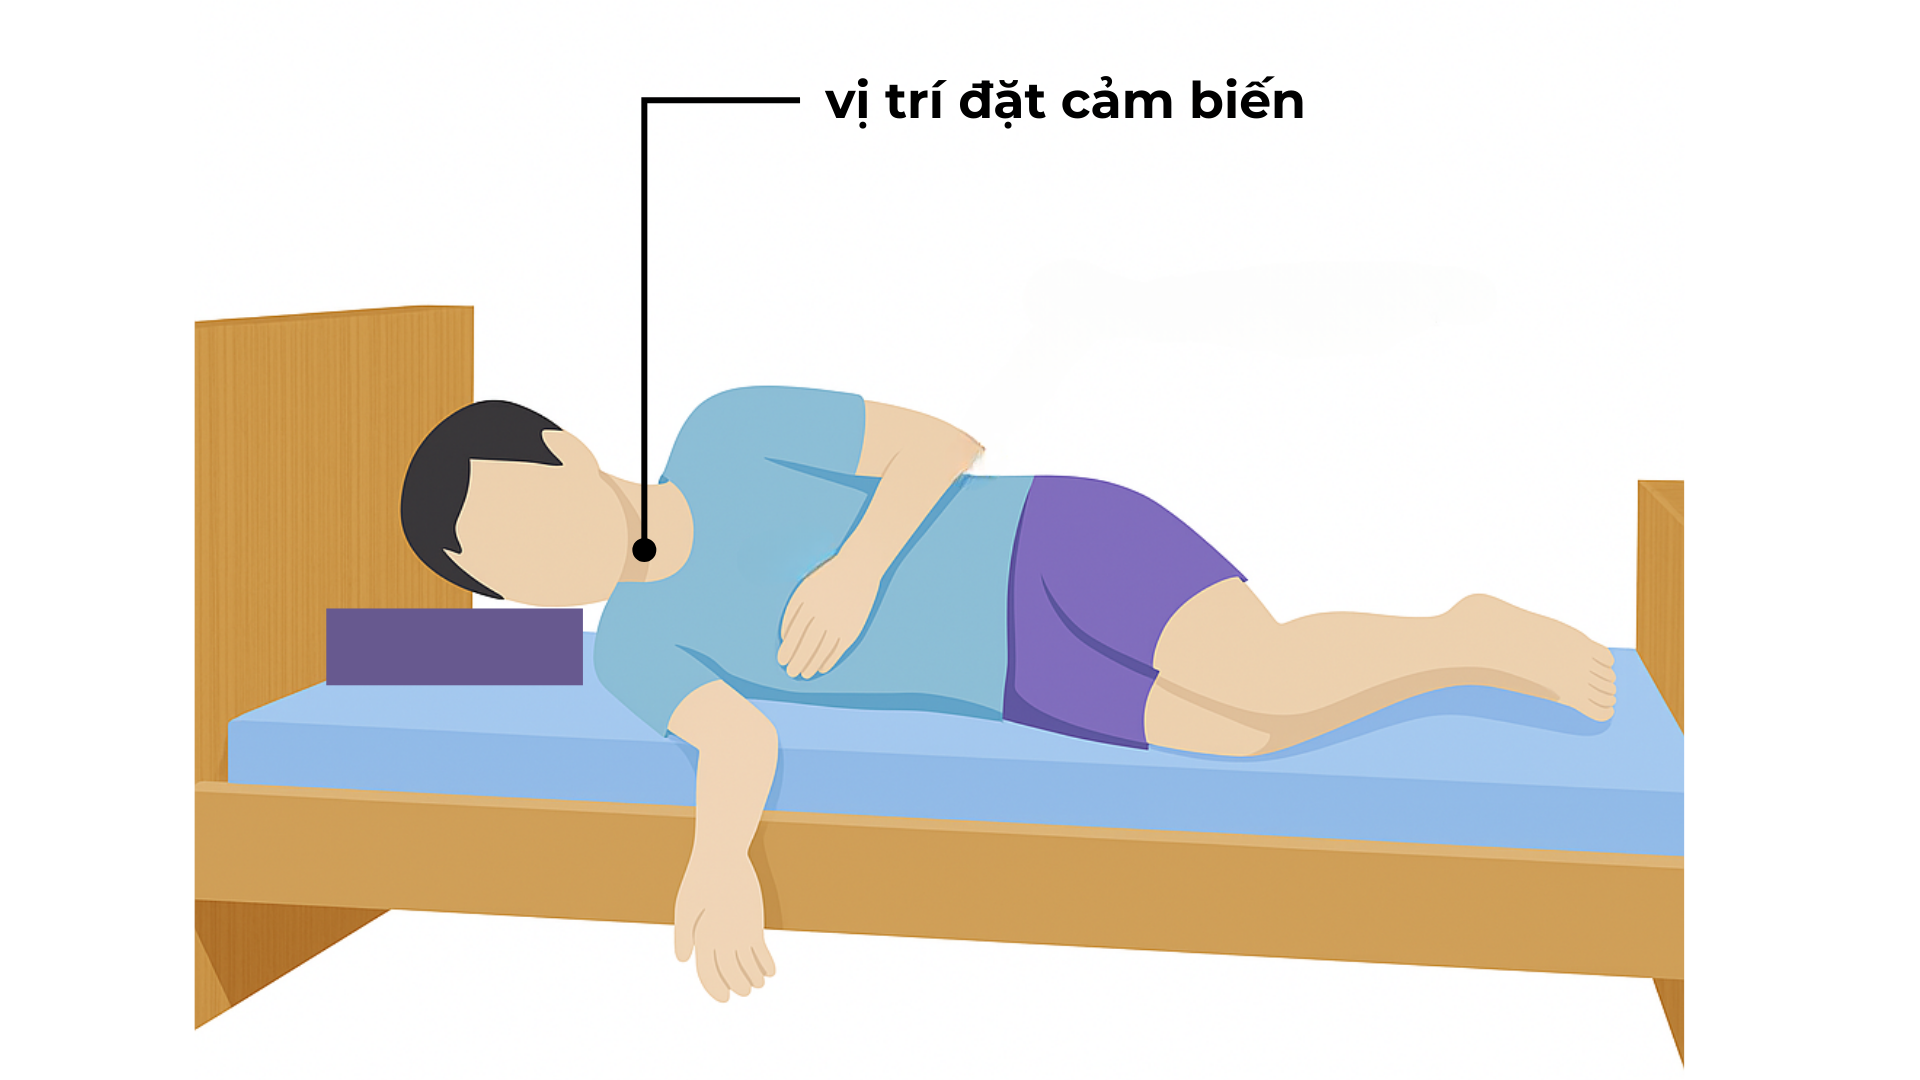
\includegraphics[width=\textwidth]{images/vị trí đặt cảm biến.png}
 		\vspace*{-7mm}
		\caption{Vị trí tối ưu để đặt cảm biến gia tốc}
		\label{position_sensor}
\end{figure}

Trong khuôn khổ luận văn, tác giả đề xuất thiết kế một thiết bị đeo tiếp xúc sử dụng cảm biến gia tốc được đặt tại vị trí xương ức cổ nhằm theo dõi và phân tích tư thế ngủ của người dùng. Vị trí này được lựa chọn không chỉ do tính ổn định trong quá trình ngủ mà còn thuận lợi để tích hợp thêm các cảm biến khác như cảm biến âm thanh và cảm biến nhiệt độ – phục vụ cho các mục tiêu nghiên cứu mở rộng của nhóm. Tín hiệu từ cảm biến gia tốc sẽ được thu thập dưới dạng ba trục không gian (x, y, z), phản ánh chuyển động và hướng trọng lực tương ứng với tư thế cơ thể trong suốt thời gian ngủ. Sau quá trình thu thập, dữ liệu gia tốc sẽ được xử lý sơ cấp bao gồm hiệu chỉnh, lọc nhiễu, và chuẩn hóa nhằm đảm bảo tính chính xác và đồng nhất giữa các mẫu đo. Tiếp theo, các đặc trưng định lượng (features) trong miền thời gian sẽ được trích xuất để phục vụ cho bài toán phân loại tư thế ngủ (ngửa, nghiêng trái, nghiêng phải, sấp). Các đặc trưng này cùng với dữ liệu gốc sẽ được lưu trữ trong hệ thống để phục vụ cho các bước phân tích tiếp theo, bao gồm huấn luyện mô hình học máy hoặc tích hợp với các chỉ số sinh lý khác trong đánh giá rối loạn giấc ngủ, đặc biệt là hội chứng ngưng thở khi ngủ (OSA) hình~\ref{position_sensor}.

\section{Giới thiệu về cảm biến gia tốc nhiều bậc tự do}
Cảm biến gia tốc (accelerometer) là thiết bị được sử dụng phổ biến để đo và phân tích gia tốc của một vật thể. Nhờ khả năng phát hiện sự thay đổi về chuyển động, cảm biến này được ứng dụng rộng rãi trong nhiều lĩnh vực như phát hiện rơi tự do, va chạm, dịch chuyển, rung động, và xoay. Nguyên lý hoạt động chính của cảm biến gia tốc dựa trên định luật II Newton (F = ma), theo đó khi một lực tác động lên một khối lượng, nó sẽ sinh ra gia tốc. Trong cấu trúc cảm biến, sự thay đổi này được ghi nhận thông qua việc chuyển đổi qua lại giữa năng lượng cơ học (sự dịch chuyển của khối lượng) và năng lượng điện (thông qua sự thay đổi điện tích, điện dung hoặc điện áp). Chính khả năng chuyển đổi năng lượng này giúp cảm biến gia tốc hoạt động hiệu quả trong việc giám sát và ghi nhận các trạng thái động học của vật thể.

\begin{figure}[!ht]
		\centering
% 		\setlength{\abovecaptionskip}{1pt plus 3pt minus 2pt}
 		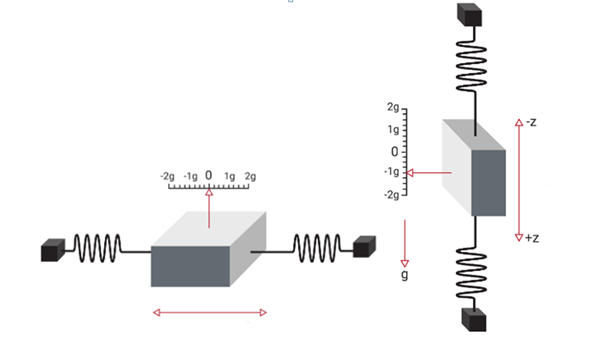
\includegraphics[width=\textwidth]{images/acce.png}
 		\vspace*{-7mm}
		\caption{Nguyên lý cơ bản của cảm biến gia tốc}
		\label{acce}
\end{figure}

Như minh họa trong Hình~\ref{acce}, khi cảm biến gia tốc chịu tác động từ một chuyển động, khối gia trọng (proof mass) sẽ dịch chuyển, làm lò xo kết nối bị biến dạng. Sự biến dạng này tạo ra một lực đàn hồi theo định luật Hooke, tỷ lệ thuận với độ giãn của lò xo. Áp dụng định luật II Newton, ta có mối quan hệ giữa lực, khối lượng và gia tốc như sau:

\begin{equation} F = m \cdot a \Rightarrow a = \frac{k \cdot \Delta l}{m} \end{equation}

Trong đó: \begin{itemize} \item $F$ là lực đàn hồi tác dụng lên khối gia trọng (N) \item $m$ là khối lượng của khối gia trọng (kg) \item $k$ là hệ số đàn hồi của lò xo (N/m) \item $\Delta l$ là độ biến dạng (thay đổi chiều dài) của lò xo (m) \end{itemize}

Phương trình trên cho thấy gia tốc có thể được tính toán gián tiếp thông qua độ biến dạng của lò xo, từ đó cho phép cảm biến gia tốc chuyển đổi dao động cơ học thành tín hiệu điện phục vụ cho việc đo đạc và phân tích chuyển động. Trong hệ tọa độ của cảm biến gia tốc ba trục, trục z thường nằm theo phương vuông góc với mặt phẳng ngang và sẽ chịu thêm tác dụng của trọng lực. Do đó, ở trạng thái cân bằng (khi thiết bị đứng yên và không có chuyển động nào khác), giá trị gia tốc đo được tại trục z sẽ xấp xỉ bằng gia tốc trọng trường $g$ (khoảng 9.81 m/s²). Đặc điểm này có thể được khai thác trong việc hiệu chuẩn cảm biến cũng như xác định tư thế không gian tương đối của thiết bị.

Trong khuôn khổ luận văn này, tác giả tập trung vào việc nghiên cứu và ứng dụng cảm biến gia tốc được chế tạo dựa trên công nghệ vi cơ điện tử (Micro-Electro-Mechanical Systems – MEMS). Đây là một công nghệ tiên tiến cho phép tích hợp các cấu trúc cơ học và linh kiện điện tử ở kích thước vi mô (dưới 10 micromet) trên cùng một chip bán dẫn. Một trong những ưu điểm vượt trội của cảm biến gia tốc MEMS là khả năng gắn trực tiếp lên bo mạch in (PCB), giúp tiết kiệm không gian, giảm chi phí sản xuất và tối ưu hóa thiết kế hệ thống nhúng – đặc biệt phù hợp với các ứng dụng trong thiết bị đeo, điện thoại di động, và hệ thống theo dõi sức khỏe cá nhân.



Hiện nay, có ba loại cảm biến gia tốc MEMS phổ biến, được phân loại dựa trên nguyên lý hoạt động của chúng \cite{Acce}\cite{cambien}:

\begin{itemize}
    \item \textbf{Cảm biến gia tốc dựa trên hiệu ứng điện dung (Capacitive accelerometers)}: Đây là loại cảm biến được sử dụng rộng rãi nhất trong các thiết bị điện tử tiêu dùng như điện thoại thông minh và thiết bị đeo. Nguyên lý hoạt động dựa trên sự thay đổi điện dung giữa các bản cực khi khối gia trọng dịch chuyển dưới tác dụng của gia tốc. Sự thay đổi điện dung này sẽ được chuyển đổi thành tín hiệu điện tương ứng với mức gia tốc.

    \item \textbf{Cảm biến gia tốc dựa trên hiệu ứng áp điện trở (Piezoresistive accelerometers)}: Trong loại cảm biến này, lực hoặc ứng suất cơ học tác động lên cảm biến sẽ làm thay đổi điện trở của vật liệu bán dẫn bên trong. Hiện tượng này – được gọi là hiệu ứng áp điện trở – có đặc tính tuyến tính, trong đó độ biến đổi của điện trở tỷ lệ thuận với lực tác động. Cảm biến loại này thường được ứng dụng trong môi trường có điều kiện khắc nghiệt, do khả năng chịu nhiệt và độ bền cao.

    \item \textbf{Cảm biến gia tốc dựa trên hiệu ứng áp điện (Piezoelectric accelerometers)}: Loại cảm biến này khai thác hiện tượng áp điện, trong đó lực cơ học tác động lên các tinh thể áp điện sẽ tạo ra điện tích. Hiệu ứng áp điện có tính tuyến tính, và lượng điện tích sinh ra tỷ lệ thuận với độ lớn của lực. Cảm biến này phù hợp trong các ứng dụng đo rung động hoặc gia tốc có tần số cao.
\end{itemize}

Mỗi loại cảm biến kể trên đều có những ưu điểm và hạn chế riêng, và việc lựa chọn loại cảm biến phù hợp phụ thuộc vào yêu cầu cụ thể của từng ứng dụng, bao gồm độ chính xác, dải đo, mức tiêu thụ điện năng và điều kiện môi trường hoạt động.



\begin{figure}[H]
	\centering
	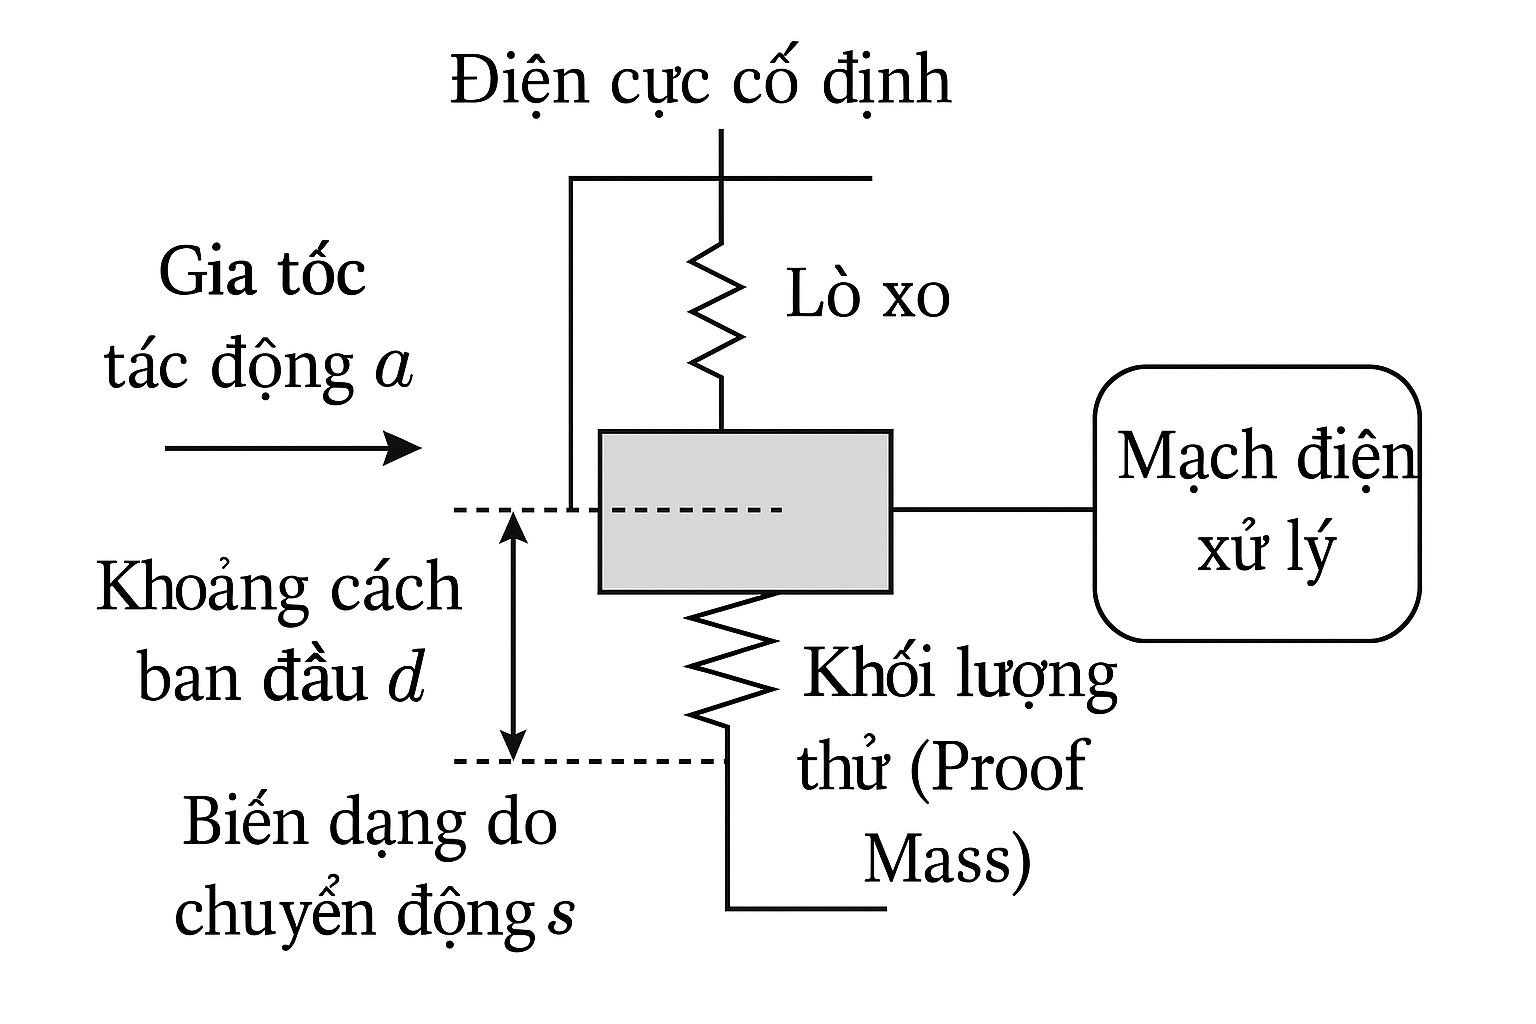
\includegraphics[width=0.7\textwidth]{images/diendung.png}
	\vspace*{-7mm}
	\caption{Cấu trúc cảm biến gia tốc điện dung}
	\label{acce_mems}
\end{figure}




\textbf{Cảm biến gia tốc kiểu điện dung (Capacitive Accelerometers)}


\textit{Nguyên lý hoạt động}: Cảm biến gia tốc kiểu điện dung hoạt động dựa trên nguyên lý biến thiên điện dung giữa các bản cực trong cấu trúc tụ điện khi chịu tác động bởi gia tốc. Cấu hình cơ bản của cảm biến bao gồm một khối lượng vi mô (proof mass) được treo trên hệ thống lò xo vi cơ (MEMS spring system), với một đầu gắn cố định và đầu còn lại liên kết với một bản cực của tụ điện. Khi có một gia tốc tác động theo một phương xác định, khối lượng này sẽ dịch chuyển lệch khỏi vị trí cân bằng, làm thay đổi khoảng cách giữa các bản cực, từ đó gây ra sự biến thiên điện dung. Biến thiên điện dung này được phát hiện thông qua mạch đo nhạy điện dung và được chuyển đổi thành tín hiệu điện tử, tỷ lệ thuận với độ lớn của gia tốc tác động. Quá trình này cho phép cảm biến thu nhận được gia tốc theo thời gian thực với độ chính xác cao. Hình~\ref{acce_mems} minh họa nguyên lý chuyển động và thay đổi điện dung trong cấu trúc cảm biến MEMS điện dung.



\begin{figure} [!]
		\centering
 		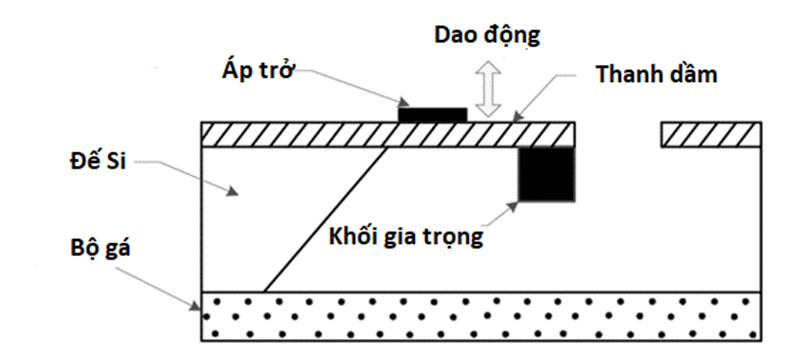
\includegraphics[width=\textwidth]{images/acce_aptro.png}
 		\vspace*{-7mm}
		\caption{Cấu trúc cảm biến áp trở}
		\label{acce_aptro}
  \FloatBarrier
\end{figure}
\textbf{Cảm biến gia tốc kiểu áp điện trở}

Cảm biến kiểu áp điện trở hoạt động dựa trên nguyên lý thay đổi điện trở của các phần tử áp điện trở khi chịu ứng suất cơ học. Trong cấu hình tiêu chuẩn, các phần tử này được gắn trên một thanh dầm (cantilever) liên kết với một khối gia trọng đặt trong môi trường cần đo. Khi có gia tốc tác động, khối gia trọng tạo ra lực quán tính khiến thanh dầm bị biến dạng, từ đó làm thay đổi điện trở của các phần tử cảm biến. Để khuếch đại và cải thiện độ chính xác của tín hiệu, các cảm biến này thường được tích hợp trong cấu trúc mạch cầu Wheatstone. Cách bố trí này cho phép tối đa hóa tín hiệu đầu ra và tăng tỷ số tín hiệu trên nhiễu (Signal-to-Noise Ratio – SNR) của phép đo (xem Hình~\ref{acce_aptro}). Gia tốc kế áp điện trở có ưu điểm nổi bật là khả năng ghi nhận các tín hiệu thay đổi chậm, cũng như hoạt động hiệu quả trong một dải đo rộng. Nhờ đó, thiết bị có thể ghi nhận các dao động có biên độ và tần số cao, rất phù hợp cho các thử nghiệm va chạm hoặc môi trường đo động học phức tạp. Ngoài ra, cảm biến này cũng cho thấy khả năng ổn định tốt trước các thay đổi nhiệt độ của môi trường xung quanh. Tuy nhiên, hạn chế chính của gia tốc kế kiểu này là độ nhạy giảm khi đo tín hiệu yếu, làm giảm hiệu quả trong một số ứng dụng yêu cầu phát hiện dao động nhỏ. Bên cạnh đó, chi phí sản xuất và triển khai cao hơn đáng kể so với các loại gia tốc kế điện dung sử dụng công nghệ MEMS.




\begin{figure} [!]
		\centering
 		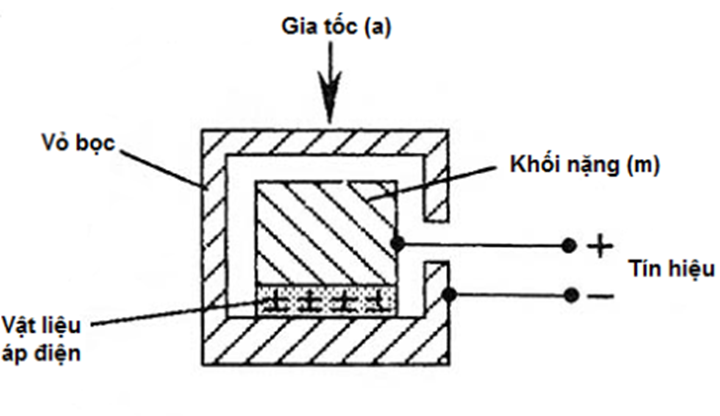
\includegraphics[width=\textwidth]{images/acce_apdien.png}
 		\vspace*{-7mm}
		\caption{Cấu trúc cảm biến áp điện}
		\label{acce_apdien}
  \FloatBarrier
\end{figure}
\textbf{Cảm biến gia tốc kiểu áp điện}

Cảm biến gia tốc kiểu áp điện hoạt động dựa trên hiệu ứng áp điện của một số vật liệu đặc biệt như gốm sứ hoặc thạch anh. Khi các vật liệu này chịu ứng suất cơ học, chúng sẽ bị biến dạng và tạo ra một điện thế trên bề mặt. Lượng điện tích sinh ra tỉ lệ thuận với lực tác dụng lên cảm biến, trong khi chiều cực tính phụ thuộc vào hướng của lực. Một trong những ưu điểm nổi bật của cảm biến gia tốc áp điện so với các loại cảm biến gia tốc khác là khối lượng nhẹ và khả năng đáp ứng tần số rất cao, có thể lên đến khoảng 1 MHz. Đặc điểm này khiến chúng đặc biệt phù hợp để đo các dao động nhanh và ngắn hạn trong các môi trường khắc nghiệt hoặc ứng dụng đòi hỏi độ chính xác cao. Tuy nhiên, cảm biến áp điện vốn có trở kháng đầu ra rất cao và chỉ tạo ra điện áp nhỏ, dễ bị suy giảm tín hiệu nếu không xử lý đúng cách. Do đó, để đảm bảo chất lượng tín hiệu và giảm thiểu hiện tượng sai số do tải (loading error), các bộ khuếch đại chuyển đổi trở kháng chuyên dụng – chẳng hạn như bộ khuếch đại điện tích – thường được tích hợp cùng hệ thống đo (xem Hình~\ref{acce_apdien}).






Đánh giá vị trí của con người trong lúc ngủ không phụ thuộc vào chuyển động quay xung quanh một trục, nên không nhất thiết phải tích hợp thêm con quay hồi chuyển. Thêm vào đó, những điểm nổi bật của cảm biến gia tốc trên công nghệ MEMS như việc ghép nối, tích hợp dễ dàng, trở kháng cao với mạch xử lý tín hiệu tích hợp sẵn cho phép đo biến đổi điện dung, độ nhạy cao, cho phép đáp ứng trong dải tần số đa dạng và đặc biệt là với chi phí phù hợp làm cho cảm biến gia tốc MEMS hay được lựa chọn trong
phát triển thiết bị ngày nay. Trong khuôn khổ luận văn này, với tính chất của chuyển động tư thế ngủ là các chuyển động chậm với biên độ nhỏ, cảm biến MEMS kiểu điện dung được lựa chọn để tiến hành thực nghiệm.

\section{Đánh giá tư thế ngủ sử dụng cảm biến gia tốc, ứng dụng công nghệ trí tuệ nhân tạo trong chẩn đoán OSA}

Vị trí là một trong bảy thông số quan trọng trong mô hình SCOPERA dùng để xác định hội chứng ngưng thở khi ngủ. Phân tích các chuyển động và tư thế trong giấc ngủ không chỉ phản ánh chất lượng giấc ngủ mà còn đóng vai trò thiết yếu trong việc đánh giá chỉ số ngưng thở – AHI. Tư thế ngủ không hợp lý có thể làm thay đổi đặc tính hô hấp và âm thanh thở, từ đó ảnh hưởng đến mức độ nghiêm trọng của OSA. Ở phần lớn bệnh nhân, mức độ nghiêm trọng của hội chứng này có xu hướng tăng rõ rệt khi họ nằm ngửa. Thống kê cho thấy, có đến 60\% bệnh nhân ghi nhận chỉ số AHI tăng gấp đôi khi ngủ ở tư thế nằm ngửa – tình trạng này được gọi là hội chứng ngưng thở khi ngủ phụ thuộc tư thế (positional Obstructive Sleep Apnea – pOSA) \cite{Unat1391}.

Vì lý do đó, việc ghi nhận và phân tích tư thế ngủ đóng vai trò then chốt trong quá trình phát triển các thiết bị hỗ trợ đánh giá giấc ngủ một cách toàn diện và chính xác. Thông tin về tư thế ngủ không chỉ góp phần làm rõ mối liên hệ giữa vị trí cơ thể và mức độ nghiêm trọng của chứng ngưng thở khi ngủ, mà còn hỗ trợ cá nhân hóa phương pháp điều trị cho từng bệnh nhân. Tư thế ngủ của con người thường được phân loại thành bốn nhóm chính: nằm ngửa, nghiêng trái, nghiêng phải và nằm sấp (Hình~\ref{4_tuthe}) \cite{4_ngu}. Việc phân biệt rõ ràng các tư thế này giúp nâng cao độ chính xác trong việc phân tích ảnh hưởng của tư thế đến các chỉ số sinh lý trong giấc ngủ.

\begin{figure}
		\centering
 		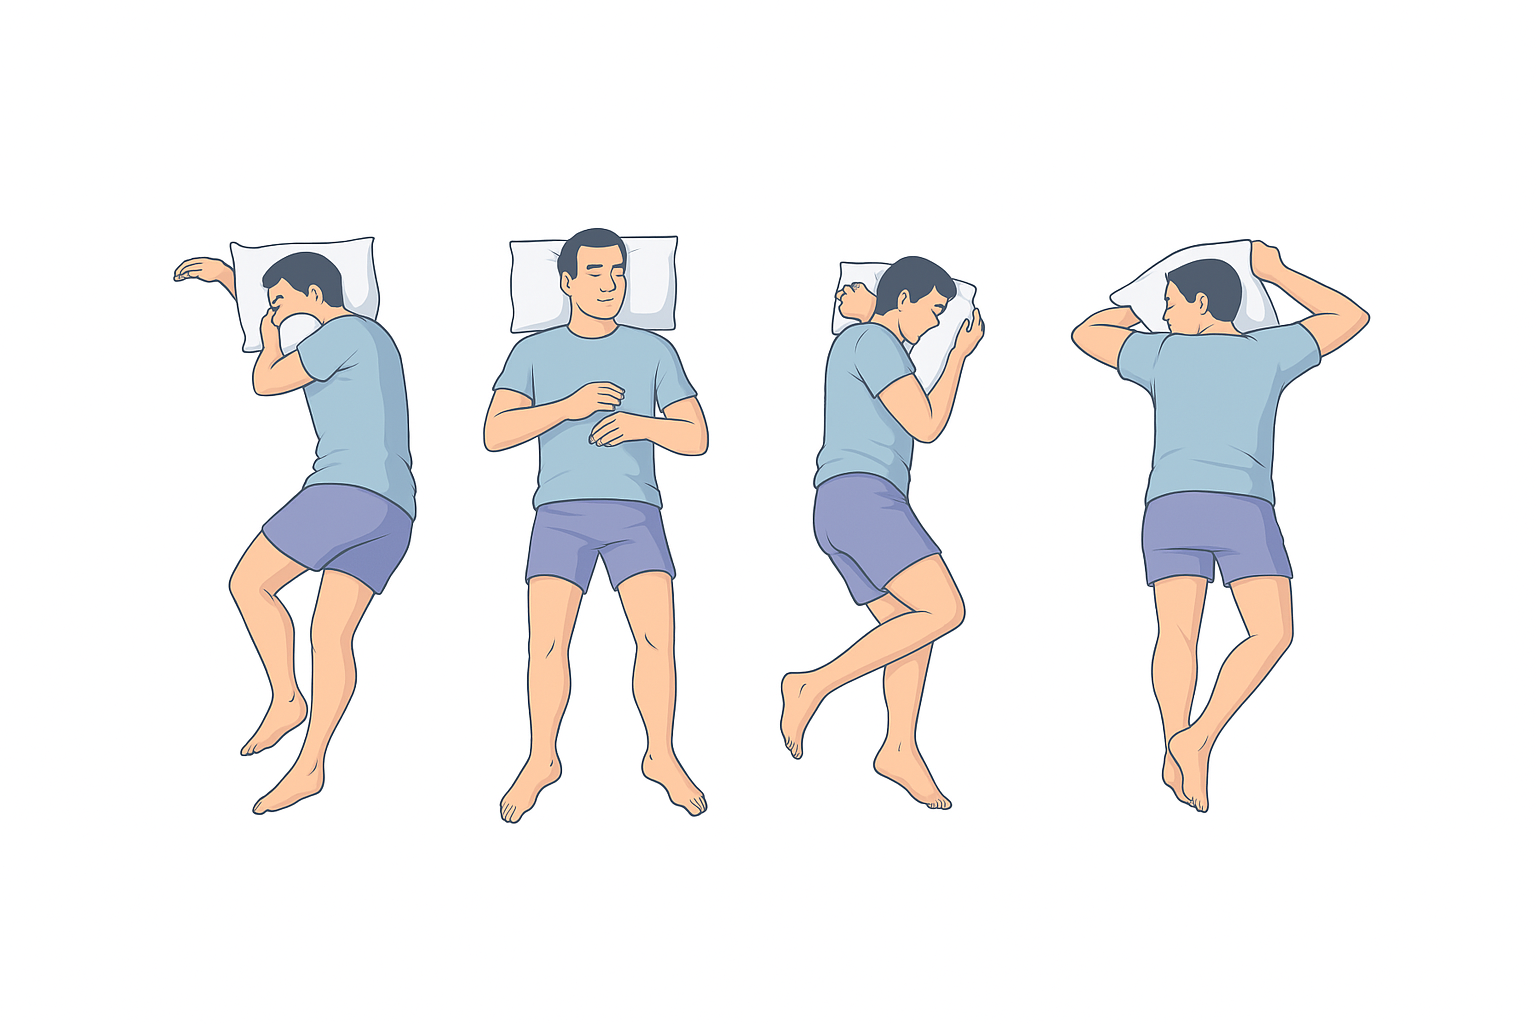
\includegraphics[width=\textwidth]{images/4ngu.png}
 		\vspace*{-7mm}
		\caption{Các tư thế ngủ cơ bản của con người}
		\label{4_tuthe}
\end{figure}

Tư thế ngủ có ảnh hưởng rõ rệt đến mức độ nghiêm trọng của hội chứng ngưng thở khi ngủ tắc nghẽn (OSA), do đó việc phân tích chi tiết từng tư thế là điều cần thiết trong các nghiên cứu và ứng dụng lâm sàng. Các tư thế ngủ khác nhau có thể tác động trực tiếp đến cơ chế tắc nghẽn đường thở, làm thay đổi tần suất và mức độ nghiêm trọng của các đợt ngưng thở. Trong số đó, các tư thế nằm nghiêng (bao gồm nghiêng trái và nghiêng phải) được ghi nhận là có khả năng cải thiện triệu chứng OSA ở nhiều bệnh nhân nhờ hạn chế tình trạng sụp đổ của đường thở trên so với tư thế nằm ngửa. Việc duy trì tư thế nằm nghiêng giúp giảm hiện tượng ngáy và hỗ trợ lưu thông khí thở tốt hơn. Tuy nhiên, sự khác biệt rõ ràng về hiệu quả giữa tư thế nghiêng trái và nghiêng phải vẫn chưa được xác định chắc chắn, và cần được đánh giá dựa trên đặc điểm cá nhân và bệnh lý kèm theo của từng người bệnh. Tư thế nằm sấp có thể làm giảm nguy cơ tắc nghẽn đường thở do trọng lực kéo các mô mềm, bao gồm cả lưỡi, về phía trước. Tuy nhiên, tư thế này không phù hợp với mọi đối tượng, đặc biệt là những người có thói quen che mặt hoặc miệng bằng gối, vì có thể làm hạn chế luồng khí hít vào. Ngoài ra, ở những bệnh nhân có vấn đề về cột sống cổ, tư thế nằm sấp có thể gây ra căng thẳng không cần thiết và làm trầm trọng thêm tình trạng cơ xương khớp. Ngược lại, tư thế nằm ngửa thường liên quan đến nguy cơ cao hơn đối với các đợt ngưng thở khi ngủ. Trong tư thế này, các mô mềm của đường thở trên – đặc biệt là lưỡi – dễ bị trọng lực kéo lùi về phía sau, gây hẹp hoặc tắc nghẽn đường thở. Do đó, nằm ngửa được xem là tư thế dễ làm trầm trọng thêm OSA và nên được cân nhắc hạn chế trong chiến lược quản lý bệnh \cite{LANDRY2023101847}.

Sự phát triển nhanh chóng của trí tuệ nhân tạo (AI) trong lĩnh vực y học đã mở ra nhiều hướng tiếp cận mới trong việc đánh giá tư thế ngủ và chẩn đoán OSA. Các hệ thống AI đang dần chứng minh hiệu quả vượt trội trong việc xử lý dữ liệu cảm biến lớn và phức tạp, từ đó cung cấp các phân tích chính xác về hành vi giấc ngủ của bệnh nhân. Các mô hình học máy được huấn luyện trên tập dữ liệu cảm biến từ accelerometer, gyroscope hoặc thiết bị đeo thông minh có thể tự động phân loại các tư thế ngủ theo thời gian thực, với độ chính xác lên đến trên 90\% trong nhiều nghiên cứu gần đây \cite{Sleep_Posture_Detection}\cite{Vu2025SleepPosition}\cite{HOANG2025116309}. 

Nhờ vào khả năng học và tự hiệu chỉnh, các thuật toán này có thể phân biệt hiệu quả giữa các trạng thái nằm nghiêng trái, nghiêng phải, nằm ngửa và nằm sấp – ngay cả khi có sự biến đổi nhẹ về góc độ hoặc cử động cơ thể. Hơn nữa, AI còn cho phép tích hợp thông tin về tư thế ngủ với các chỉ số sinh lý khác như nhịp tim, nhịp thở, SpO₂ và dữ liệu âm thanh để xây dựng mô hình chẩn đoán OSA đa chiều. Việc kết hợp các nguồn dữ liệu này giúp phát hiện chính xác các giai đoạn ngưng thở và giảm thở, đồng thời đánh giá được mức độ ảnh hưởng của từng tư thế đến tình trạng hẹp đường thở trong khi ngủ. Đây là một bước tiến quan trọng hướng đến cá nhân hóa chẩn đoán và điều trị OSA – điều mà các phương pháp truyền thống như đa ký giấc ngủ (polysomnography) còn nhiều hạn chế do chi phí cao và điều kiện thực hiện phức tạp. Đặc biệt, các hệ thống AI có thể được triển khai trong các thiết bị đeo thông minh tại nhà, hỗ trợ theo dõi lâu dài và liên tục mà không gây xâm lấn hay gián đoạn giấc ngủ. Nhờ đó, dữ liệu thu thập được phản ánh chính xác hơn về hành vi giấc ngủ trong môi trường tự nhiên của người bệnh, từ đó nâng cao giá trị lâm sàng của các kết quả phân tích. Ngoài ra, sự tích hợp AI trong các thiết bị di động, cùng với công nghệ điện toán biên (edge computing), có thể cho phép xử lý dữ liệu tại chỗ và phản hồi thời gian thực – mở ra tiềm năng to lớn trong việc sàng lọc, theo dõi và cá nhân hóa chiến lược quản lý OSA.

















% \section{Cơ chế giả lập hành vi\label{mock_mechanism}} 
% % Từ khóa sử dụng: mock, mocking, mock data, HTTP Request, caller, callee, API method
% \begin{lstlisting}[float,language=JavaScript,caption={Ví dụ phương thức API ($searchMasterData()$) gọi đến hai phương thức khác, trong đó có một phương thức ($get()$) cần được tạo hàm giả khi thực thi kiểm thử}, label=api_example,captionpos=b]
async get(req: RequestModel): Promise<any> { //Accessing database (*@\label{declare_get_method}@*)
    return await this.httpService
      .post<any>(Utils.join(this.apiUrl, this.config.CORE_GET), req) (*@\label{call_http_service}@*)
      .toPromise(); (*@\label{get_method_toPromise}@*)}
      
@Post('search') //The tested API
async searchMasterData(@Body() body: RequestModel<BaseDto>): Promise<any> { (*@\label{declare_api_method}@*)
    // Hidden code...
    await this.checkRequired(body.condition['type']); (*@\label{lst_exp_check_require}@*)
    let reqCon = body.condition;
    switch (reqCon['type']) { (*@\label{lst_exp_switch_stmt}@*)
        case "MASTER":(*@\label{lst_exp_case_branch}@*)
            if (!(type of reqCon["keyword"] === "string") (*@\label{lst_exp_if_stmt}@*)) {
                (*@\label{lst_exp_keyword_branch}@*)return ResponseModel(RESULT_STATUS.ERROR);}
            const ret = await this.get(reqCon);(*@\label{lst_exp_start_uncover}@*)
            if (ret.status == 200) { (*@\label{lst_exp_200}@*) 
                // Hidden code... (*@\label{lst_exp_hidden_code}@*)
                return  new ResponseModel(RESULT_STATUS.OK, ret); (*@\label{lst_exp_end_uncover}@*)}
            return new ResponseModel(RESULT_STATUS.ERROR);(*@\label{lst_exp_return_error}@*)
        //Other cases....
        default: (*@\label{lst_exp_default_branch}@*)
            return new ResponseModel(RESULT_STATUS.ERROR);}
}

checkRequired(s: string): Promise<any> { //A normal method (*@\label{declare_check_required_method}@*)
    if (s == null (*@\label{check_null_equal}@*)) {
        this.errors.push("error message");}
}
\end{lstlisting}

% \begin{lstlisting}[float,language=JavaScript,caption={An example presents one caller ($search()$) and two callees ($get()$ and $check()$), in which the first callee ($get()$) needs to be mocked.}, label=api_example,captionpos=b]
% @Post('search')
% async search(body: Dto): any { (*@\label{declare_api_method}@*)
%     this.check(body['type']); (*@\label{lst_exp_check_require}@*)
%     switch (body['type']) { (*@\label{lst_exp_switch_stmt}@*)
%         case "MASTER":(*@\label{lst_exp_case_branch}@*)
%             if (body["keyword"] is not a string)(*@\label{lst_exp_if_stmt}@*)) 
%                 return ...
%             const ret = await this.get(reqCon);(*@\label{lst_exp_start_uncover}@*)
%             if (ret.status == 200 (*@\label{lst_exp_200}@*)) 
%                 return ... (*@\label{lst_exp_end_uncover}@*)
%             else  return ...(*@\label{lst_exp_return_error}@*)
%     }
% }
% //A method gets data from database
% async get(req): any (*@\label{declare_get_method}@*){ ...}
% check(s: string): any (*@\label{declare_check_required_method}@*) {  //A normal callee
%     if (s == null (*@\label{check_null_equal}@*))  
%         this.errors.push("error message");}
% \end{lstlisting}
% % return await this.httpService
% %       .post<any>(Utils.join(this.apiUrl, this.config.CORE_GET), req) (*@\label{call_http_service}@*).toPromise(); (*@\label{get_method_toPromise}@*)
% \begin{lstlisting}[float,language=JavaScript,caption=An example of mocking $get()$ method, label=mock_example,captionpos=b]
% it("first test", (done) => {
%     // generated input
%     const body = {...}; (*@\label{input_declaration}@*)
%     // initialize mock data
%     const response: AxiosResponse < any > = {(*@\label{mock_declare_response}@*) status: 200,
%         data: {}, headers: {}, statusText: 'OK', config: {url:'x'}};
%     // set mock data to method accessing database
%     jest.spyOn(controller_class, "get").mockResolvedValue(response); (*@\label{mock_spy}@*)
%     // call the tested API
%     return request(server).post("/search") (*@\label{begin_test_driver}@*)
%     .send(body)  (*@\label{end_test_driver}@*).expect(201).then(res => {...})
% });
% \end{lstlisting}
% Quá trình thực thi kiểm thử cần được đảm bảo là độc lập và nhanh chóng \cite {clean_coder}. Để làm được điều này, chúng ta có thể áp dụng cơ chế giả lập hành vi cho một số hàm hoặc phương thức tương tác với thành phần bên ngoài như cơ sở dữ liệu, dịch vụ bên thứ ba, v.v. Cơ chế giả lập hành vi (\textit{\gls{mocking}}) được sử dụng để cài đặt các hàm hoặc phương thức với các hành vi mới. Thay vì truy cập các tài nguyên từ xa như trang Web hoặc cơ sở dữ liệu, các nhà phát triển hoặc người kiểm thử có thể thay thế hành vi mới của hàm/phương thức bằng cách sử dụng dữ liệu giả (\textit{\gls{mockdata}}). \Gls{mockdata} được cố ý chèn vào một phần trong mã nguồn. Nó thường được sử dụng như là kết quả của các phương thức hoặc hàm. Nó có nghĩa là những phương thức/hàm này được thay đổi hành vi để phù hợp với việc thực thi kiểm thử. Để đơn giản, thuật ngữ \textit {``\gls{mocked_method}"} dùng để chỉ một phương thức kết nối với các tài nguyên từ xa và phải được thay đổi hành vi. Sử dụng cơ chế \gls{mocking} có hai lợi ích chính là quá trình kiểm thử trở nên nhanh chóng và độc lập, điều này cần có trong các nguyên tắc FIRST \cite {clean_coder}. 

% Ưu điểm đầu tiên của việc sử dụng cơ chế \gls{mocking} là nhanh chóng. Kỹ thuật này làm giảm chi phí tính toán để thực thi dữ liệu thử nghiệm. Nếu không áp dụng cách thức này, việc kết nối với các tài nguyên từ xa có thể gặp phải một số sự cố do kết nối mạng kém hoặc không khả dụng. Thay vì đợi phản hồi từ các tài nguyên từ xa, các phương thức có thể trả về nhanh chóng \gls{mockdata}. Một lợi thế khác của việc sử dụng cơ chế \gls{mocking} là đảm bảo tính độc lập. Nó giúp duy trì tính nhất quán của cơ sở dữ liệu khi thực thi dữ liệu thử nghiệm nhiều lần. Khi một ứng dụng Web doanh nghiệp được triển khai, hầu hết các API có thể yêu cầu một số thay đổi tương tác với cơ sở dữ liệu. Tuy nhiên, trong môi trường thử nghiệm, việc thực thi thử nghiệm không được tác động đến cơ sở dữ liệu để duy trì tính nhất quán của dữ liệu gốc. Thay vì thực hiện hành vi thực tế, các phương thức có thể trả về \gls{mockdata} ngay lập tức. Do đó, việc thực thi thử nghiệm sẽ không bao giờ thực hiện bất kỳ cập nhật nào đối với cơ sở dữ liệu.

% Để làm rõ hơn cơ chế \gls{mocking} được sử dụng như thế nào trong thực tế, ví dụ trong Mã nguồn~\ref{api_example} và Mã nguồn~\ref{mock_example} thể hiện một trường hợp cần phải dùng tới cơ chế này. Ví dụ đầu tiên Mã nguồn~\ref{api_example} có API $``/search"$ lấy dữ liệu từ tài nguyên bên ngoài bằng cách gọi phương thức $get()$ (dòng \ref{lst_exp_start_uncover}). Bên cạnh đó, Mã nguồn~\ref{mock_example} trình bày một ca kiểm thử có sử dụng \gls{mocking} cho API $``/search"$  trong Mã nguồn~\ref{api_example}. 
% Để đơn giản hóa, nếu phương thức $m_1$ gọi phương thức $m_2$, $m_1$ và $m_2$ tương ứng được gọi là
% \textit{``caller"} và \textit{``callee"}.

% \begin{lstlisting}[float,language=JavaScript,caption=Ví dụ áp dụng \gls{mocking} đối với mã nguồn dự án sử dụng framework NestJS, label=mock_example,captionpos=b]
it("first test", (done) => {
    const body = {...}; (*@\label{input_declaration}@*)  // input generated by the two methods
    const response: AxiosResponse < any > = {(*@\label{mock_declare_response}@*)// initialize mock data
        data: {}, headers: {}, config: {},
        status: 200, statusText: 'OK'};
    // set mock data to method accessing database
    jest.spyOn(controller_class, "get")
        .mockResolvedValue( of(response).toPromise()); (*@\label{mock_spy}@*)
    // send request data to the tested API
    return request(server)
    .post("/search") (*@\label{begin_test_driver}@*)
    .send(body)  (*@\label{end_test_driver}@*)
    .expect(201).then(res => {
        console.log(res.body);
        expect(res.body).not.toBeNull();
        done();
    })
});
\end{lstlisting}
% Thứ nhất, Mã nguồn~\ref{api_example} thể hiện một ví dụ cần phải sử dụng cơ chế \gls{mocking} khi thực thi kiểm thử. Ví dụ này có một phương thức chính ($searchMasterData()$) và hai phương thức phụ ($get()$ và $checkRequired()$). Chúng là những đại diện điển hình của mã nguồn dự án được sử dụng làm thực nghiệm trong Mục~\ref{experiment_section} Mỗi phương thức đều có những đặc điểm riêng biệt. Đầu tiên, phương thức chính ($searchMasterData()$) được đánh dấu với ký hiệu $@Post("search")$ cung cấp bởi thư viện NestJS (dòng \ref{declare_api_method}). Điều này có nghĩa là phương thức này tương ứng với một API. API này có thể được lựa chọn nằm trong môi trường kiểm thử. Phương thức này gọi tới hai phương thức khác: phương thức $get()$ để lấy kết quả phản hồi từ một cơ sở dữ liệu (dòng \ref{lst_exp_start_uncover}) và phương thức thứ hai $checkRequired()$ để kiểm tra lại tính hợp lệ của dữ liệu đầu vào (dòng \ref{lst_exp_check_require}). 
% Ngoài ra, phương thức đầu tiên ($get()$) kết nối với máy chủ cơ sở dữ liệu từ xa bằng cách sử dụng đối tượng $httpService$ với phương thức $post()$ để gửi POST Request (dòng \ref{call_http_service}). Phương thức này cần được thiết lập hành vi giả trong tệp kiểm thử. Liên quan đến vấn đề này, kiểu trả về của phương thức này có cấu trúc lớp $AxiousResponse$ bao gồm một số thuộc tính như là $data, headers,config, status$, và $statusText$ \footnote{https://github.com/axios/axios\#response-schema}. Những thuộc tính này cần được cung cấp trong \textit{mock data} để thỏa mãn yêu cầu về kiểu trả về của phương thức. Cuối cùng, phương thức $checkRequired()$ là một phương thức bình thường có nhiệm vụ là kiểm tra sự tồn tại của một thuộc tính đặc biệt trong đầu vào. Vì vậy, nó không cần thiết phải áp dụng cơ chế \gls{mocking} trong tệp thực thi kiểm thử.
% % The caller is an API that needs to be tested and it calls the callee which connects to a remote database.
% % As a result, the consistency of data could be impacted during test execution. Therefore, the actual implementation of this callee has to be replaced by using mock data

% Thứ hai, Mã nguồn~\ref{mock_example} trình bày ví dụ một tập lệnh cho một ca kiểm thử cho API $@Post("search")$ trong Mã nguồn~\ref{api_example}. Tập lệnh này có sử dụng cơ chế \gls{mocking} cho phương thức truy cập đến có sở dữ liệu  $get()$. Đây là ví dụ một khối lệnh viết bằng ngôn ngữ Typescript để xây dựng một ca kiểm thử cho một API trong ứng dụng NestJS. API được gọi với đầu là một HTTP Request có chứa dữ liệu kiểm thử ảnh hưởng đến luồng thực thi của chương trình. Khối lệnh này có cấu trúc bao gồm ba phần: Khai báo giá trị đầu vào (dòng \ref{input_declaration}), khai báo \textit{mock data}  (dòng \ref{mock_declare_response}-\ref{mock_spy}), và lời gọi API (dòng \ref{begin_test_driver}-\ref{end_test_driver}).
% Như đã đề cập ở trước đó, phương thức $get()$ kết nối tới máy chủ cơ sở dữ liệu và cần được thiết lập hành vi thay thế. Vì vậy, \textit{mock data} được cung cấp (dòng \ref{mock_declare_response}-\ref{mock_spy}). Ở khía cạnh đầu tiên, nếu cơ chế \gls{mocking} không được áp dụng, phương thức $get()$ sẽ gửi một POST Request tới máy chủ từ xa dẫn đến tốn thêm thời gian để đợi phản hồi. Thêm vào đó, nếu máy chủ đang không khả dụng, giá trị thuộc tính $status$ của biến $ret$ trong Mã nguồn~\ref{api_example} luôn luôn khác $200$. Điều này có nghĩa là biểu thức điều kiện $ret.status == 200$ luôn luôn nhận giá trị $false$ (dòng \ref{lst_exp_200} trong Mã nguồn~\ref{api_example}), khiến một số câu lệnh không thể được thực thi khi chạy kịch bản kiểm thử (dòng \ref{lst_exp_hidden_code},\ref{lst_exp_end_uncover} trong Mã nguồn~\ref{api_example}). 
% Ở khía cạnh khác, cơ chế \gls{mocking} cần được áp dụng để đảm bảo cơ sở dữ liệu không bị ảnh hưởng (dòng \ref{mock_spy}). \Gls{mockdata} của phương thức $get()$  là giá trị của biến $response$ bao gồm tất cả những thuộc tính cần thiết như là $data, headers,config, status$, và $statusText$ (dòng \ref{mock_declare_response}). Những giá trị này sẽ giúp chương trình thực thi nhiều câu lệnh hơn. 

% Trên thực tế, \gls{mockdata} thường được các nhà phát triển hoặc người thử nghiệm sửa đổi dựa trên kinh nghiệm của họ. Bởi vì luồng thực thi có thể phụ thuộc vào cách các phương thức được giả lập, \gls{mockdata} có thể ảnh hưởng đến phạm vi bao phủ. Do đó, các nhà phát triển hoặc người kiểm tra cần phải hiểu rõ ràng về mã nguồn để thiết lập \gls{mockdata} phù hợp nhằm đạt được độ phủ cao hơn.

% \section{Kiểm thử ứng dụng Web}
% Cách đơn giản nhất để kiểm thử một ứng dụng Web là kiểm thử viên sẽ thực hiện các thao tác nhấp chuột thủ công trên giao diện của hệ thống và đánh giá cách ứng dụng phản hồi. Đây là phương pháp kiểm thử hộp đen \cite{black_box_testing} vì kiểm thử viên không cần biết chi tiết nội hàm của chương trình ứng dụng. Họ chỉ cần quan tâm xem với một đầu vào cụ thể, ứng dụng có thực thi hành vi đúng như đặc tả hay không. Phương pháp kiểm thử này dễ dàng thực hiện được vì không cần bất cứ thiết lập nào trước đó. Tuy nhiên, nó có thể bị ảnh hưởng bởi những lỗi liên quan đến người thực hiện kiểm thử. Ngoài ra, quá trình này cũng tốn rất nhiều thời gian và công sức khi mà tổ hợp các kịch bản người dùng thực hiện trên giao diện là một con số rất lớn. Điều này trở nên thách thức hơn khi mã nguồn luôn luôn có sự thay đổi, quá trình kiểm thử hồi quy cần được thực hiện liên tục để kiểm tra lại các thành phần trước đó vẫn hoạt động đúng như ban đầu. Vì vậy, việc kiểm thử đầy đủ nếu chỉ dựa vào kiểm thử thủ công trên giao diện là không hiệu quả.

% Thay vì kiểm thử viên nhấp chuột thủ công để kiểm thử hệ thống, họ có thể viết các dữ liệu kiểm thử sử dụng trình điều khiển Web. Trình điều khiển Web thực hiện lần lượt các bước mô tả trong dữ liệu kiểm thử và kiểm tra hành vi của hệ thống. Quá trình thực thi các dữ liệu kiểm thử này có thể được tự động hóa cho nên nó có thể tiết kiệm thời gian cho kiểm thử viên ở giai đoạn thực thi hệ thống. Những dữ liệu kiểm thử có thể được tái sử dụng cho những lần kiểm thử hồi quy sau này. Tuy nhiên, về bản chất, việc xây dựng và viết mã lệnh cho các dữ liệu kiểm thử vẫn phải thực hiện thủ công. Đây là công việc rất tốn thời gian và nguồn nhân lực, đòi hỏi lập trình viên có kiến thức về trình điều khiển Web. Để kiểm thử đầy đủ cho một ứng dụng Web, số lượng dữ liệu kiểm thử là rất lớn. Vì vậy, trong thực tế, danh sách dữ liệu kiểm thử thường không đầy đủ dẫn đến một số lỗi tiềm ẩn trong chương trình không thể phát hiện và thường bị bỏ qua.

% Với những hạn chế như đã được để cập ở trên, việc sinh dữ liệu kiểm thử cần được tự động hóa sao cho đảm bảo tính hiệu quả để tiết kiệm thời gian và chi phí cho doanh nghiệp phát triển phần mềm. Đây cũng là một trong những mảng nghiên cứu khá là quan trọng, dành được nhiều sự quan tâm của các nhà nghiên cứu trong lĩnh vực công nghệ phần mềm. Việc kiểm thử cho ứng dụng Web hiện nay gặp phải một số thách thức \cite{web_testing_1, web_testing_2}. Hiện tại, quá trình nghiên cứu các phương pháp tự động hóa sinh dữ liệu kiểm thử cho ứng dụng Web cũng đã đạt được một số kết quả nhất định. Có thể kể đến một số dự án nổi bật như là Artemis\cite{artermis}, Crawljax \cite{crawljax}, và SymJS \cite{symjs}. Artemis là một công cụ hỗ trợ kiểm thử tự động cho ứng dụng Javascript, tập trung vào các ứng dụng đơn trang. Công cụ này sử dụng một số hằng số và giá trị ngẫu nhiên để sinh ra đầu vào cho dữ liệu kiểm thử. Tiếp theo, Crawljax là một công cụ thu thập thông tin và kiểm thử cho các ứng dụng Web Ajax. Nó có thể thực hiện trên ứng dụng Web có quy mô lớn nhưng chỉ sinh ra các giá trị ngẫu nhiên cho đầu vào. Cả hai công cụ này mặc dù có thể sinh dữ liệu kiểm thử tự động cho ứng dụng Web nhưng bộ dữ liệu kiểm thử không hiệu quả vì không phân tích sâu đến nội hàm các xử lý lô-gic của thành phần kiểm thử. Khác với hai công cụ trước đó, SymJS là công cụ có phân tích mã nguồn của thành phần kiểm thử trong ứng dụng, thu thập các toán tử có điều kiện và thực thi tượng trưng để sinh ra bộ các đầu vào đi qua các đường đi khác nhau trong chương trình. Tuy nhiên, hiện tại công cụ này mới chỉ hỗ trợ mã nguồn JavaScript phía người dùng. Có thể nói rằng SymJS đã bước đầu nghiên cứu các phương pháp kiểm thử hộp trắng cho các ứng dụng Web. Phương pháp kiểm thử hộp trắng từ lâu đã được ứng dụng để sinh tự động dữ liệu kiểm thử ở nhiều ngôn ngữ lâu đời như Java, C++, C\#, v.v. và đã đạt được một số kết quả khả quan. Bộ dữ liệu kiểm thử được sinh ra bởi phương pháp này có thể đạt độ phủ cao, thực thi qua nhiều thành phần có trong chương trình. Tuy nhiên, phương pháp này cũng vẫn tồn tại mộ số nhược điểm nhất định và chưa thể coi như là một giải pháp tổng thể cho tất cả các mã nguồn dự án phần mềm. Việc áp dụng phương pháp này như thế nào thì phải phụ thuộc vào bài toán cụ thể hoặc đặc trưng của mã nguồn được áp dụng. Thời điểm hiện tại vẫn chưa có nhiều nghiên cứu ứng dụng phương pháp kiểm thử hộp trắng cho ứng dụng Web.

% \section{Kiểm thử hộp trắng}
% Phương pháp được đề xuất trong luận văn này xây dựng dựa trên phương pháp kiểm thử dòng điều khiển. Đây là một trong những phương pháp kiểm thử hộp trắng đảm bảo tất cả các thành phần có trong mã nguồn đều được thực thi. Cụ thể, kiểm thử hộp trắng là phương pháp sinh dữ liệu kiểm thử dựa trên việc phân tích cấu trúc bên trong của mã nguồn \cite{software_testing, white_box_testing_2}. Nếu kiểm thử hộp đen cho phép phát hiện lỗi/khiếm khuyết có thể quan sát được thì kiểm thử hộp trắng có thể phát hiện những lỗi/khiếm khuyết tiềm ẩn bên trong chương trình/đơn vị phần mềm. Các lỗi này thường rất khó có thể phát hiện bằng kiểm thử hộp đen, tuy nhiên điều này không có nghĩa là kiểm thử hộp đen là không quan trọng. Mỗi phương pháp đều có những ưu nhược điểm và mục đích khác nhau, thường xuyên được sử dụng kết hợp với nhau trong quy trình kiểm thử nhằm đảm bảo phần mềm có chất lượng tốt nhất. Kiểm thử hộp trắng có các dữ liệu kiểm thử được sinh ra từ mã nguồn bằng các kỹ thuật phân tích phức tạp. Vì vậy, để có thể áp dụng được phương pháp này, các kỹ thuật viên không chỉ cần nắm rõ giải thuật mà còn cần có các kỹ năng và kiến thức tốt về ngôn ngữ lập trình, hiểu rõ được mã nguồn mới có thể đưa ra những cách giải quyết phù hợp. Do đó, việc áp dụng các phương pháp kiểm thử hộp trắng thường tốn nhiều thời gian và công sức, đặc biệt khi thành phần kiểm thử có kích thước lớn. Với lý do như vậy, các phương pháp kiểm thử hộp trắng thường được áp dụng trong pha kiểm thử đơn vị.

% Hai phương pháp được sử dụng trong kiểm thử hộp trắng là kiểm thử dòng điều khiển (Control Flow Testing - CFT) và kiểm thử dòng dữ liệu (Data Flow Testing - DFT) \cite{whitebox-testing}. Phương pháp kiểm thử dòng điều khiển tập trung kiểm thử tính đúng đắn của các giải thuật sử dụng trong thành phần cần kiểm thử. Phương pháp kiểm thử dòng dữ liệu quan tâm đến tính đúng đắn của việc sử dụng các biến dữ liệu trong thành phần kiểm thử. Luận văn này sử dụng phương pháp kiểm thử dòng điều khiển. Vì vậy, các kiến thức liên quan đến kiểm thử dòng điều khiển được trình bày chi tiết trong phần tiếp theo.
% % cần kiểm thử nhưng vẫn phát hiện được lỗi ngay từ giai đoạn đầu tiên trong quy trình phát triển phần mềm. Nhờ đó, các khiếm khuyết trong thiết kế và code được sửa chữa sớm, giảm thời gian và chi phí hoàn thiện sản phẩm. Đồng thời, hiệu suất phát triển cũng được nâng cao vì thiết kế được cải tiến, code có chất lượng tốt hơn, dễ bảo trì. Ngoài việc kiểm tra tài liệu (code reviews) và đánh giá cú pháp tự động, kiểm thử hộp trắng có thể được ứng dụng trong việc sinh dữ liệu kiểm thử thỏa mãn những tiêu chí đánh giá về độ phủ. Cụ thể trong phạm vi khóa luận này, phương pháp kiểm thử hộp trắng được áp dụng là xây dựng đồ thị luồng điều khiển đại diên cho cấu trúc chương trình và sử dụng tiêu chuẩn bao phủ nhánh của đồ thị để làm căn cứ đánh giá sự hiểu quả của giải pháp. 

% % % \section{Cây cú pháp trừu tượng}
% % % Cây cú pháp trừu tượng (Abstract Syntax Tree - AST) được sử dụng rộng rãi trong các trình biên dịch hoặc IDE. Với đầu vào là mã nguồn, các trình biên dịch/IDE này sẽ xây dựng AST tương ứng. AST là một cách biểu diễn cấu trúc mã nguồn dưới dạng cây. Mỗi một thành phần trong cây tương ứng với một thành phần mã nguồn như câu lệnh gán, khối lệnh điều kiện, biến, phép toán, v.v. Đối với một ngôn ngữ bất kỳ, AST
% % % Mỗi thành phần trong cây đều có các kiểu khác nhau được quy định bởi trình biên dịch. Ví dụ, trong CDT, kiểu IASTDeclSpecifier tương ứng với kiểu trả về của hàm hay kiểu biến. Kiểu IASTBinaryExpression tương ứng với dấu phép toán. Kiểu IASTName đại diện tên biến, tên hàm. IASTReturnStatement chính là câu lệnh return. 
% \section{Đồ thị dòng điều khiển}
% Như đã giới thiệu, phương pháp được sử dụng trong luận văn này là kiểm thử dựa trên dòng điều khiển. Tổng quan của phương pháp này là phân tích mã nguồn, xây dựng đồ thị dòng điều khiển và phân tích các biểu thức điều kiện có trong đồ thị đề sinh ra các giá trị hữu ích. Việc sinh dữ liệu kiểm thử dựa trên phân tích mã nguồn sẽ gặp rất nhiều khó khăn nếu chỉ thao tác với mã nguồn ở dạng văn bản đơn thuần. Vì vậy, chúng ta cần có một cấu trúc dữ liệu khác cũng có thể mô tả mã nguồn nhưng đơn giản để phân tích hơn. Đồ thị dòng điều khiển là một cấu trúc dữ liệu hỗ trợ giải quyết vấn đề này. Đồ thị dòng điều khiển (Control Flow Graph - \gls{CFG}) mô tả kịch bản thực thi của chương trình một cách trực quan, bao gồm các đỉnh là đại diện cho câu lệnh/nhóm câu lệnh và các cạnh là dòng điều khiển giữa các câu lệnh/nhóm câu lệnh đó \cite{CFG_definition}. Tất cả các đồ thị luồng điều khiển đều có đỉnh bắt đầu và đỉnh kết thúc đại diện cho trạng thái bắt đầu và trạng thái kết thúc của chương trình. Các cạnh là các mũi tên có hướng thể hiện thứ tự thực hiện của câu lệnh/nhóm câu lệnh. Cạnh nối hai đỉnh $i$ và $j$ theo hướng từ đỉnh $i$ đến đỉnh $j$ nghĩa là câu lệnh thứ $i$ được thực hiện trước câu lệnh thứ $j$.
% Về cơ bản, CFG bao gồm các thành phần chính là đỉnh bắt đầu, đỉnh xử lý, đỉnh quyết định, đỉnh kết nối và đỉnh kết thúc. 
% \begin{itemize}
%     \item Đỉnh bắt đầu: Đánh dấu thời điểm bắt đầu của chương trình, được thể hiện bằng hình tròn
%     \item Đỉnh xử lý: Đại diện cho các câu lệnh gán, khai báo và khởi tạo, được thể hiện bằng hình chữ nhật
%     \item Đỉnh quyết định: Đại diện cho câu lệnh điều khiển trong khối lệnh điều khiển rẽ nhánh, được thể hiện bằng hình thoi
%     % \item Đỉnh kết nối: Đại diện cho câu lệnh được thực hiện ngay sau các lệnh rẽ nhánh, có nhiều hơn hai đỉnh trỏ đến, được thể hiện bằng hình tròn
%     \item Đỉnh kết thúc: Đánh dấu thời điểm kết thúc của hàm, được thể hiện bằng hình tròn
% \end{itemize} 
% \begin{figure}[!ht]
% 		\centering
% % 		\setlength{\abovecaptionskip}{1pt plus 3pt minus 2pt}
%  		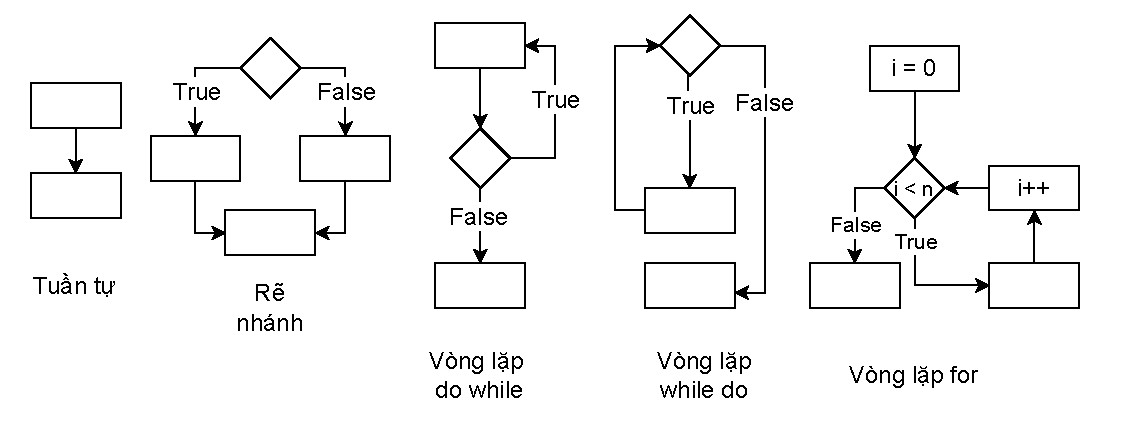
\includegraphics[width=\textwidth]{figures/cfg-control.pdf}
%  		\vspace*{-7mm}
% 		\caption{Các cấu trúc điều khiển phổ biến trong TypeScript}
% 		\label{cau-truc-dieu-khien}
% \end{figure}

% Hình~\ref{cau-truc-dieu-khien} mô tả các cấu trúc điều khiển chính có trong TypeScript được mô phỏng dưới dạng các đỉnh của CFG, bao gồm có cấu trúc điều khiển tuần tự, rẽ nhánh, vòng lặp \textit{for}, vòng lặp \textit{do…while}, vòng lặp \textit{ while…do}.

% \section{Các độ đo kiểm thử}
% Các độ đo kiểm thử thường được xác định là các quy tắc hoặc yêu cầu mà một tập hợp dữ liệu kiểm thử cần đáp ứng \cite{coverage_criteria}. Có một số độ đo phổ biến là bao phủ hàm (function coverage), bao phủ câu lệnh (statement coverage) và bao phủ nhánh (branch coverage). Bao phủ hàm là độ đo dễ đạt được nhất trong ba tiêu chí bao phủ này. Nó được đo bằng tỷ lệ phần trăm các hàm hoặc phương thức đã thực thi trên tổng số các hàm/phương thức có trong mã nguồn thử nghiệm. Bởi vì một hàm được thực thi có thể chứa các đoạn chưa được thực thi như các câu lệnh và các nhánh, một số lỗi bên trong một hàm có thể không được xem xét. Để giải quyết vấn đề này, quá trình kiểm tra phải được thực hiện với cả phạm vi bao phủ của câu lệnh và phạm vi bao phủ nhánh. Liên quan đến bao phủ câu lệnh, nó được biểu thị bằng tỷ lệ phần trăm các câu lệnh được thực thi trong tổng số các câu lệnh thuộc phạm vi kiểm thử. Nếu độ phủ câu lệnh đạt 100\%, thì bao phủ hàm/phương thức cũng đạt đến 100\%. Tuy nhiên, nó không thể xác nhận rằng tất cả các nhánh của điều kiện đều được thực thi. Vì vậy, độ phủ nhánh được đề xuất để đánh giá quá trình thử nghiệm một cách toàn diện hơn. Nó được đo bằng phần trăm các nhánh được thực thi trên tất cả các nhánh thuộc phạm vi kiểm thử. Nếu việc thực thi kiểm thử đạt được bao phủ nhánh tối đa, có thể đảm bảo rằng bao phủ câu lệnh và hàm cũng đạt đến giá trị lớn nhất. Vì vậy, bao phủ nhánh được sử dụng là độ đo cơ bản để đánh giá bộ dữ liệu kiểm thử.

% Công thức tổng quát để tính độ phủ theo các độ đo của $n$ tệp được trình bày trong Công thức \ref{coverage_equation}:
% \begin{equation} \label{coverage_equation}
% \begin{split}
%         e_c &= f(c, tested\ files) \\
%         &= \frac{\sum_{i=1}^n e_{i_c}}
%         {\sum_{i=1}^n t_{i_c}}*100 \\
%  \end{split}
% \end{equation}
% ,trong đó: $c$: loại độ đo bao phủ, bao gồm bao phủ hàm (\textit{function coverage}), bao phủ câu lệnh (\textit{statement coverage}), bao phủ nhánh (\textit{branch coverage})\\
% $e_{i_c}$: số lượng các thành phần được thực thi theo từng độ đo $c$ trong tệp thứ $i$. Thành phần được coi là các hàm, câu lệnh, và nhánh trong mã nguồn kiểm thử. \\
% $t_{i_c}$: số lượng tất cả các thành phần theo độ đo $c$ trong tệp thứ $i$

% Các tiêu chí bao phủ này được sử dụng để đánh giá hiệu quả của phương pháp được đề xuất trong việc tạo dữ liệu thử nghiệm. Nếu độ phủ tăng lên, nhiều thành phần trong mã nguồn được thực thi. Trong trường hợp các độ phủ không đạt 100 \%, các vấn đề sau có thể gặp phải. Thứ nhất, dữ liệu kiểm thử không thực thi toàn bộ các thành phần có trong mã nguồn. Do đó, có thể có một số lỗi tiềm ẩn không được phát hiện. Mặt khác, mã nguồn có thể chứa những câu lệnh không bao giờ có thể thực thi. Các nhà phát triển phải loại bỏ những đoạn mã này để tối ưu kích thước chương trình, tránh thực hiện các hành vi không đúng hoặc đơn giản hóa cấu trúc chương trình.

% % Trong kiểm thử hộp trắng nói chung và kiểm thử dòng điều khiển nói riêng, bài toán kiểm thử là sinh được bộ dữ liệu kiểm thử sao cho thỏa mãn các tiêu chuẩn cho trước. Các tiêu chuẩn này đã được thống nhất và định nghĩa bằng văn bản trong ISO \cite{iso_coverage}. Công thức tính toán độ đo theo các tiêu chuẩn này dựa trên mức độ bao phủ của chương trình với một tập dữ liệu kiểm thử cho trước. Tập dữ liệu kiểm thử có độ phủ cao sẽ đáng tin cậy hơn tập dữ liệu kiểm thử có độ phủ thấp. Mục tiêu là tập dữ liệu kiểm thử có số lượng tối thiểu nhưng đạt được độ phủ tối đa. Hiện nay, có nhiều tiêu chuẩn bao phủ khác nhau được sử dụng. Độ phủ của mỗi tiêu chuẩn đánh giá đều có công thức tính riêng nhưng về cơ bản sẽ được tính bằng tỉ lệ thành phần được kiểm thử trên tổng số các thành phần cần kiểm thử. Thành phần ở đây có thể là câu lệnh, nhánh chương trình, điểm quyết định, điều kiện con hoặc sự kết hợp giữa chúng. Độ đo này giúp các kỹ thuật viên kiểm soát và quản lý quá trình kiểm thử tốt hơn, có thể kiểm tra lại thành phần không được chạy qua hoặc bổ sung thêm dữ liệu kiểm thử trong trường hợp độ phủ thấp. Dưới đây là ba độ đo kiểm thử được sử dụng nhiều trong quy trình kiểm thử phần mềm \cite{Lee03}.
% % \begin{itemize}
% %     \item Độ phủ câu lệnh (statement coverage): mỗi câu lệnh được đi qua ít nhất một lần sau khi chạy bộ dữ liệu kiểm thử.
% %     \item Độ phủ nhánh (branch coverage): nhánh đúng và nhánh sai của mỗi đỉnh điều kiện có trong đồ thị dòng điều khiển được đi qua ít nhất một lần sau khi chạy bộ dữ liệu kiểm thử.
% %     \item Độ phủ điều kiện con (Modified Condition/Decision Coverage - MC/DC): các điều kiện con thuộc các đỉnh điều kiện phức tạp đều được thực hiện cả hai nhánh đúng và nhánh sai ít nhất một lần mỗi nhánh sau khi chạy bộ dữ liệu kiểm thử.
% % \end{itemize}

% % \section{Đường kiểm thử}
% % Bộ dữ liệu kiểm thử sinh ra dành cho một hàm bao gồm nhiều dữ liệu kiểm thử. Mỗi dữ liệu kiểm thử là một bộ giá trị đầu vào của tham số. Với một bộ giá trị đầu vào, chương trình của hàm sẽ chạy qua một số câu lệnh và dừng lại khi tới điểm kết thúc. Tập hợp các câu lệnh theo thứ tự thực hiện tạo thành một đường đi. Những đường đi được chọn để sinh dữ liệu kiểm thử  được gọi là đường kiểm thử. Để thống nhất khái niệm sử dụng trong suốt khóa luận, Định nghĩa 2.4 mô tả tổng quát một đường kiểm thử. Mỗi đường kiểm thử có thể bao gồm đầy đủ các câu lệnh khai báo, gán giá trị, khởi tạo và câu lệnh rẽ nhánh. Các đường đi khác nhau sẽ khác nhau ở số lượng, danh sách và thứ tự thực hiện các câu lệnh. Việc sinh dữ liệu kiểm thử tương ứng với đường kiểm thử chính là tìm kiếm bộ giá trị đầu vào sao cho khi thực thi, các nút điều kiện của đường đi đều được thỏa mãn. Trong thực tế, số lượng đường đi của chương trình có thể rất lớn dẫn đến việc sinh bộ dữ liệu kiểm thử cho tất cả các đường đi là không thể. Vì vậy, một số đường đi được chọn để sinh dữ liệu kiểm thử nhằm đáp ứng tiêu chí về độ phủ được gọi là tập đường kiểm thử.\\
% % \textbf{Định nghĩa 2.1}: Đường kiểm thử là một đường đi từ điểm bắt đầu đến điểm kết thúc của CFG, được biểu diễn bằng tập hợp các đỉnh từ $v_1$  đến $v_n$ sao cho cứ hai đỉnh cạnh nhau thì có cạnh nối theo hướng từ trái qua phải. Nếu cạnh ($v_i$, $v_j$) là nhánh sai thì biểu thức điều kiện tại đỉnh $v_i$ được viết dưới dạng phủ định $!v_i$.

% % Để có thể sinh được bộ dữ liệu kiểm thử thỏa mãn yêu cầu về tiêu chuẩn bao phủ, việc lựa chọn tập kiểm thử là một công đoạn không thể thiếu. Tuy nhiên, có hai vấn đề chúng ta cần phải đối mặt:
% % \vspace{-0.5cm}
% % \begin{itemize}
% %     \item Tính khả thi của đường đi: Một đường kiểm thử gọi là có khả khi nếu tồn tại một dữ liệu kiểm thử sao cho khi thực thi trong môi trường thật, tất cả các đỉnh của đường đi được duyệt qua. Ngược lại, đường kiểm thử gọi là không khả thi.
% %     \item 	Sự bùng nổ đường đi: với một hàm có kích thước lớn, nhiều vòng lặp hoặc các lệnh rẽ nhánh phức tạp, số lượng đường đi của chương trình có thể rất lớn. Việc sinh dữ liệu kiểm thử cho tất cả các đường đi để chắc chắn đạt độ phủ 100\% là không thể.
% % \end{itemize}
% % Mục tiêu của khóa luận này là xây dựng công cụ đầu tiên hỗ trợ sinh dữ liệu kiểm thử cho TypeScript, bắt đầu thử nghiệm với các hàm TypeScript kích thước vừa phải. Vì vậy, tập đường kiểm thử được lựa chọn là tập các đường đi có thể có của chương trình. Trong trường hợp tất cả các đường đi đều khả thi, độ bao phủ nhánh có thể đạt được là 100\%.

% % \section{Thư viện sử dụng}

% % \subsection{Thư viện phân tích mã nguồn TypeScript ``ts-morph''}
% % Phương pháp sinh dữ liệu kiểm thử tự động được đề xuất trong khóa luận này dựa trên việc thao tác với CFG của hàm. Việc xây dựng CFG như thế nào sẽ tùy biến theo từng tình huống bài toán. Đặc biệt đối với một ngôn ngữ mới như TypeScript, hiện tại không có thư viện nào có thể hỗ trợ giải quyết tác vụ này. Vì vậy, quá trình này được thực hiện thủ công dựa trên kỹ thuật phân tích mã nguồn và thiết kế cấu trúc dữ liệu mô hình hóa sao cho phù hợp với bài toán kiểm thử hiện tại. Phân tích mã nguồn thành cây cú pháp trừu tượng (Abstract Syntax Tree - AST) giúp việc xây dựng CFG trở nên đơn giản hơn. AST là một cây đại diện cho cấu trúc cú pháp trừu tượng của mã nguồn. Ngôn ngữ lập trình khác nhau có AST khác nhau.  Mỗi nút của cây biểu thị một cấu trúc có trong mã nguồn. AST thường được xây dựng bởi chính trình phân tích cú pháp của ngôn ngữ tương ứng trong quá trình biên dịch. Đối với các ngôn ngữ lâu đời, việc này có thể được thực hiện bởi một số thư viện khác. Do TypeScript là một ngôn ngữ mới nên chưa có công cụ nào hỗ trợ phân tích mã nguồn thành AST. Vì vậy, khóa luận này sử dụng chính trình biên dịch ngôn ngữ TypeScript của Microsoft để phân tích nội dung hàm. ``ts-morph''\footnote{\url{https://github.com/dsherret/ts-morph}} là một thư viện mở rộng từ trình biên dịch TypeScript, cung cấp các giao diện lập trình ứng dụng (Application Programming Interface - API) hỗ trợ người dùng có một cách dễ dàng hơn để điều hướng chương trình và thao tác với mã TypeScript.
% % Với sự hỗ trợ của ``ts-morph'', người sử dụng có đầy đủ các API để trích xuất thông tin cần thiết từ mã nguồn.  Các khối lệnh của thân hàm và các biểu thức  điều kiện đều có thể dễ dàng có được thông qua việc duyệt các đỉnh, hay gọi là $node$ của AST. Ngoài ra, thư viện cung cấp giao diện\footnote{\url{https://TypeScript-ast-viewer.com/}} để người dùng có thể theo dõi kết quả dưới dạng hình cây rất trực quan và dễ nhìn. Từ đó, việc thao tác với AST trở nên dễ dàng hơn.

% % %  Đối với TypeScript, các cấu trúc này có thể là lớp, hàm, thuộc tính, tham số, câu lệnh, v.v.

% % \subsection{Bộ giải hệ ràng buộc Z3}
% % Công cụ sinh dữ liệu kiểm thử cho mỗi đường kiểm thử bằng cách giải hệ ràng buộc ứng với tập các đỉnh điều kiện. Giải hệ ràng buộc nghĩa là quá trình tìm ra giải pháp cho một tập hợp các ràng buộc áp đặt bởi các phép toán điều kiện mà các biến phải thỏa mãn \cite{ref-constraints}. Do đó, một giải pháp là một tập hợp các giá trị cho các biến thỏa mãn tất cả các ràng buộc, đó là một điểm trong vùng khả thi.
% % Hiện nay, có nhiều thư viện, công cụ hỗ trợ việc giải hệ trong đó nổi bật là bộ giải Z3. Bộ giải Z3 được xây dựng chủ yếu bằng ngôn ngữ C++. Các ràng buộc cần được chuyển sang dạng chuẩn của Z3 để công cụ có thể tính toán và giải nghiệm. Z3 có thể giải hệ ràng buộc của các số nguyên, số thực, mảng và hàm tượng trưng. Đặc biệt trong phiên bản 4.8, bộ giải Z3 hỗ trợ giải một số ràng buộc liên quan đến chuỗi (string) \cite{z3_str_paper}. Điều này giúp việc tìm kiếm dữ liệu kiểm thử có tham số đầu vào kiểu chuỗi trở nên đơn giản hơn. Để có thể sử dụng Z3 giải nghiệm, bộ ràng buộc được lưu trong tệp và khởi chạy tiến trình bằng dòng lệnh:
% % \vspace{0.5cm}
% % \begin{lstlisting}
% % z3 -smt2 <file name>.smt2
% % \end{lstlisting}
% % Mã nguồn~\ref{constraints-file-example} là ví dụ một tệp constraints.smt2 hợp lệ làm đầu vào cho bộ giải Z3. Trong tệp, các biến sử dụng cần được khai báo bằng cú pháp \textit{declare-fun}. Sau đó, lệnh \textit{assert} được sử dụng để thêm các ràng buộc của hệ. Để kiểm tra hệ ràng buộc có nghiệm hay không, lệnh \textit{check-sat} được gọi. Kết quả trả về là \textit{sat} nếu có nghiệm và \textit{unsat} trong trường hợp không có nghiệm. Tập các giá trị của các biến thỏa mãn hệ ràng buộc được hiển thị bằng lệnh \textit{get-model}. Trong ví dụ này, hệ ràng buộc sử dụng ba biến tham số đầu vào là tvw\_s,  tvw\_a, tvw\_b và có ba ràng buộc được thêm vào câu lệnh \textit{assert} trong tệp \textit{constraints.smt2}. Mã nguồn~\ref{z3-result-example} là kết quả tương ứng sau khi giải hệ. Trong đó, các giá trị của các biến tìm được là  tvw\_a = 12,  tvw\_b = 11,  tvw\_s = "\textbackslash x00\textbackslash x00\textbackslash x00\textbackslash x00\textbackslash x00". Như vậy, bộ giá trị (a, b, s) = \{12, 11, "\textbackslash x00\textbackslash x00\textbackslash x00\textbackslash x00\textbackslash x00"\} là một nghiệm của hệ ràng buộc.
% % Nếu áp dụng với một đường kiểm thử cụ thể, các biến được khai báo trong hệ ràng buộc là các biến gọi đến trong các câu lệnh. Các đỉnh điều kiện sẽ được biểu diễn qua những biến này và chuẩn hóa thành những ràng buộc của hệ. Kết quả giải hệ là một dữ liệu kiểm thử thỏa mãn đường đi tương ứng. Trong trường hợp hệ ràng buộc của tất cả các đường đi đều giải được bỏi bộ giải Z3, tập các dữ liệu kiểm thử thu được phủ 100\% đường đi của CFG.

% % \vspace{0.5cm}
% % \begin{lstlisting}[caption=Ví dụ nội dung tệp đầu vào cho bộ giải Z3, label=constraints-file-example,captionpos=b]
% % (set-option :timeout 5000)
% % (declare-fun tvw_s () String)
% % (declare-fun tvw_a () Int)
% % (declare-fun tvw_b () Int)
% % (assert (> a b))
% % (assert (> b 10))
% % (assert (not (> (+ (str.len tvw_s) 1) 10)))
% % (check-sat)
% % (get-model)
% % \end{lstlisting}

% % \begin{lstlisting}[caption=Ví dụ kết quả giải hệ của Z3, label=z3-result-example, captionpos=b]
% % sat
% % (model
% %   (define-fun tvw_s () String
% %     "\x00\x00\x00\x00\x00")
% %   (define-fun tvw_b () Int
% %     11)
% %   (define-fun tvw_a () Int
% %     12)
% % )

% % \end{lstlisting}

% % \subsection{Mocha và Istanbul}
% % Để kiểm tra độ phủ đạt được với bộ dữ liệu kiểm thử đã được sinh tự động, công cụ có sử dụng Mocha trong việc thực thi mã nguồn. Mocha (Mocha Test Framework) là một bộ công cụ hỗ trợ kiểm thử dành cho JavaScript giàu tính năng chạy trên Nodejs và trong trình duyệt, giúp cho việc kiểm tra bất đồng bộ trở nên đơn giản và thú vị \cite{ref-mocha}. Các quy trình thực thi kiểm thử thực hiện bởi Mocha chạy ổn định, cho phép báo cáo linh hoạt và chính xác. Mocha có thể áp dụng với TypeScript thông qua một số bước cài đặt kỹ thuật. Ngoài ra,  Mocha cũng có thể kết hợp với một số thư viện để xuất báo cáo kiểm tra độ phủ (test coverage report). Ngoài việc cung cấp chức năng chạy kiểm thử với thao tác bằng tay, Mocha còn kèm theo bộ API để vận hành các bài kiểm tra tự động. Mocha có rất nhiều tính năng tuyệt vời, trong đó có một số tính năng nổi bật được kể đến là:
% % \begin{itemize}
% %     \item Hỗ trợ bất đồng bộ đơn giản
% %     \item Cung cấp đa dạng báo cáo
% %     \item Có thể chạy trong trình duyệt
% %     \item Tương thích với nhiều thư viện xác nhận (assertion library) Javascript
% %     \item Tương thích với mô hình phát triển phần mềm định hướng hành vi (Behaviour Driven Development - BDD) và mô hình phát triển phần mềm định hướng kiểm thử (Test Driven Development - TDD)
% % \end{itemize}
% % Với sự hỗ trợ của Mocha, các tệp kiểm thử được thực thi một cách nhanh chóng. Kết quả chạy kiểm thử được thống kê trực quan với số lượng dữ liệu kiểm thử thành công hay thất bại kèm theo vị trí cụ thể. Từ đó kỹ thuật viên nhanh chóng xác định được dữ liệu kiểm thử bị sai và dễ dàng sửa chữa.

% % Mocha chỉ hỗ trợ quá trình thực thi tệp kiểm thử và thống kê kết quả số lượng dữ liệu kiểm thử thành công hay thất bại. Tuy nhiên, để có thể biết được thống kê độ phủ mà bộ dữ liệu kiểm thử đạt được, Mocha cần kết hợp thêm một số thư viện bên ngoài. trong đó, được sử dụng nhiều nhất phải kể đến thư viện Istanbul \cite{ref-instanbul}. Đây là thư viện hỗ trợ sinh báo cáo độ phủ của quá trình kiểm thử đơn vị với nhiều định dạng khác nhau như HTML, XML, terminal output, JSON, v.v. Người dùng có thể lựa chọn kiểu báo cáo phù hợp với nhu cầu. Công cụ được phát triển trong khóa luận sử dụng báo cáo thể hiện dưới dạng HTML, bao gồm các thông tin về các độ phủ như số lượng hàm, câu lệnh, nhánh được thực thi. Đồng thời, báo cáo cũng nổi bật các đoạn mã không được chạy qua. Từ đó, kỹ thuật viên có thể phát hiện ra  được các đoạn mã không bao giờ được chạy để làm sạch mã nguồn hoặc bổ sung thêm dữ liệu kiểm thử mới để bộ dữ liệu kiểm thử hoàn thiện hơn.